%%%%%%%%%%%%%%%%%%%%%%%%%%%%%%%%%%%%%%%%%%%%%%%%%%%%%%%%%%
%                                                                                      %
%         Bristol Project LaTex Template            %
%                                                                                      %
%%%%%%%%%%%%%%%%%%%%%%%%%%%%%%%%%%%%%%%%%%%%%%%%%%%%%%%%%%
%
%   Author: Alex Charles           Email: aep.charles@gmail.com
%
% -----------------------------------------------------------------------------------
%      PACKAGES & OTHER DOCUMENT CONFIGURATIONS
% -----------------------------------------------------------------------------------
\documentclass[fontsize=9.5pt]{extarticle}

\usepackage[utf8]{inputenc}
\usepackage[T1]{fontenc}
\usepackage[british]{babel}
% ----------NEW BIBLATEX BIBLIOGRAPHY-----------------------------------------------
\usepackage[eprint=false,backend=bibtex,style = ieee]{biblatex} % Upgrades Bibliography Block Ragged helps break lines in url fixes error

\addbibresource{BibFile.bib} %%% For biblatex
%e.g to add page number \footfullcite[chapter, p.~215]{AAIB}
% This allows can use footfullcite commands
% Note urldate field must be in yyyy-mm-dd to work - use online type
% Remeber to use \printbibliography in the footer
% -----------------------------------------------------------------------------------
% \usepackage{sectsty}
\usepackage{url}

%%% --- The following two lines are what needs to be added --- %%%
\setcounter{biburllcpenalty}{7000}
\setcounter{biburlucpenalty}{8000}

\usepackage{amssymb,amsmath}
\numberwithin{figure}{section} %%%%% <<<<<< Puts Figure Numbering into Sections
\usepackage{ifxetex,ifluatex}  %<<<<<<<<< Edit FONT HERE
% \usepackage{fontspec}
% \setmainfont{Times New Roman}
\ifnum 0\ifxetex 1\fi\ifluatex 1\fi=0 % if pdftex
  \usepackage[T1]{fontenc}
  \usepackage[utf8]{inputenc}
\else % if luatex or xelatex
  \ifxetex
    \usepackage{mathspec}
    \setmainfont[
 BoldFont={AvenirNext-Medium},ItalicFont={AvenirNext-Italic},
 BoldItalicFont={AvenirNext-MediumItalic}]{AvenirNext-Regular}
  \else
  % Font Package for XeLatex
    \usepackage{fontspec}
    \setmainfont{AvenirNext-Regular}
  \fi
  \defaultfontfeatures{Ligatures=TeX,Scale=MatchLowercase}
\fi
\usepackage[fit]{truncate} %Truncates headers that are too long
\usepackage[headheight=26pt,headsep=0.15cm]{geometry}
\usepackage{fancyhdr}
\usepackage{lastpage}
\usepackage{extramarks}
\usepackage{gensymb}
\usepackage{lipsum}
\usepackage{float}
\usepackage{graphicx}
\graphicspath{{TempImg/}{Img/}}%<<<<<<<<< Location of Template Images and Other Images, Add folders here
\usepackage{subfig}
\usepackage{wrapfig}
\usepackage[font ={small,it}]{caption}
\usepackage{amsfonts,amsthm} % Math packages
% \usepackage{cite}
\usepackage{csquotes}
%    \MakeAutoQuote{‘}{’}
%    \MakeAutoQuote*{“}{”} %corrects quote marks
\usepackage{enumitem} % resume numbered lists
\usepackage{multicol} %for mulitple colums in lists
\usepackage{booktabs} %<<<<<<<<< Table drawing package
\usepackage[table,xcdraw]{xcolor} %<<<<<<<<< Table drawing package
\usepackage{svg}
\usepackage{scrextend} %call footnotes
\usepackage[colorlinks, linkcolor = black, citecolor = black, filecolor = black, urlcolor = blue]{hyperref} % Creates Hyperlinks for references - add [colorlinks] for coloured hyperlinks
\usepackage{changepage} %Allows Adjust width to be used for the document (indenting paragraphs)
\usepackage{pdfpages} %Allows Pdfpages to be added to the document use \includepdf[pages={1}]{myfile.pdf}
\usepackage{pdflscape} %Change Pages from Portrait to Landscape
\usepackage{color,soul} %% Highlights text for markup
% \usepackage[compact]{titlesec}
\usepackage{titlesec}
\titlespacing\section{0pt}{6pt plus 2pt minus 2pt}{0pt plus 2pt minus 2pt}
\titlespacing\subsection{0pt}{0pt plus 3pt minus 2pt}{-3pt plus 2pt minus 2pt}
\titlespacing\subsubsection{0pt}{0pt plus 2pt minus 2pt}{-6pt plus 2pt minus 2pt}
\titlespacing\subsubsubsection{0pt}{-6pt plus 2pt minus 2pt}{-6pt plus 2pt minus 2pt}
\setlength{\multicolsep}{-1pt plus 2.0pt minus 1.5pt}% 50% of original values

% \titlespacing*{\section}{0pt}{1.1\baselineskip}{\baselineskip}

\renewcommand*{\thefootnote}{\alph{footnote}} %%% Changes footnotes to letters
\usepackage[bottom]{footmisc} %%% Pushes footnote to bottom and to the margin

\DeclareCiteCommand{\footcite}[\mkbibfootnote]
{\usebibmacro{cite:init}%
\usebibmacro{prenote}}
{\usebibmacro{citeindex}%
\printtext[brackets]{\usebibmacro{cite:comp}}}
{\multicitedelim}
{\usebibmacro{cite:dump}%
\usebibmacro{postnote}}

\newenvironment{indentpara}{\begin{adjustwidth}{2cm}{}}{\end{adjustwidth}} %Declare adjust width wiht indentpara
\renewcommand{\labelitemii}{$\circ$}
\renewcommand{\labelitemiii}{$\diamond$}
\renewcommand{\labelitemiii}{$\cdot$}

% -----------------------------------------------------------------------------------
%                 Code
% -----------------------------------------------------------------------------------
\usepackage{listings}
\lstset{inputpath=Code/}
\usepackage{color}
\definecolor{mygreen}{RGB}{28,172,0} % color values Red, Green, Blue
\definecolor{mylilas}{RGB}{170,55,241}

\lstset{language=Matlab,%
    %basicstyle=\color{red},
    breaklines=true,%
    basicstyle=\small,
    morekeywords={matlab2tikz},
    keywordstyle=\color{blue},%
    morekeywords=[2]{1}, keywordstyle=[2]{\color{black}},
    identifierstyle=\color{black},%
    stringstyle=\color{mylilas},
    commentstyle=\color{mygreen},%
    showstringspaces=false,%without this there will be a symbol in the places where there is a space
    numbers=left,%
    numberstyle={\tiny \color{black}},% size of the numbers
    numbersep=9pt, % this defines how far the numbers are from the text
    emph=[1]{for,end,break},emphstyle=[1]\color{red}, %some words to emphasise
    %emph=[2]{word1,word2}, emphstyle=[2]{style},
}

%% To Add Code Use :
% \lstinputlisting{myfun.m}
%% To input a file or :
% \begin{figure}[h]
% \begin{lstlisting}[language=Matlab]
% \end{lstlisting}
% \catpion{code}
% \end{figure}


% -----------------------------------------------------------------------------------
%                 Quotes
% -----------------------------------------------------------------------------------

\usepackage{epigraph}
% \epigraphsize{\small}% Default
\setlength\epigraphwidth{12cm}
\setlength\epigraphrule{0pt}

\usepackage{etoolbox}
\apptocmd{\sloppy}{\hbadness 10000\relax}{}{}%%%% > Removes Url bibliography warnings
\makeatletter
\patchcmd{\epigraph}{\@epitext{#1}}{\itshape\@epitext{#1}}{}{}
\makeatother

%%%% > For Quotes Use \epigraph{"Quote"}{ - \textup{Author}, Book}

% -----------------------------------------------------------------------------------
%                   NAMES & CLASS DEFINITION %<<<<<<<<< INSERT DETAILS HERE
% -----------------------------------------------------------------------------------
\newcommand{\AssignmentTitle}{Investigation of the Use Energy Storage Technologies to Reduce Peak Demand Charges for the University of Bristol New Campus}
\newcommand{\ModuleTitle}{Design Project 4 - Final Report}
\newcommand{\University}{University of Bristol}
\newcommand{\Faculty}{Faculty of Engineering}
\newcommand{\UniCrest}{crestbris.png}
\newcommand{\UniLogo}{logobris.png}%<<<<<<<<< Make Sure Files are in the Template
%\newcommand{\GroupName}{Group 2}
\newcommand{\StudentNameA}{Alexander Charles}
\newcommand{\StudentNumberA}{67634}
\newcommand{\SupervisorNameA}{Dr Theo Tryfonas}
\newcommand{\SupervisorEmailA}{Theo.Tryfonas@bristol.ac.uk}
% \newcommand{\SupervisorNameB}{Name}
% \newcommand{\SupervisorEmailB}{email@gmail.com}

% -----------------------------------------------------------------------------------
%        PACKAGES FOR MARKDOWN CONVERSION - FOR USE If Using Markdown to Latex
% -----------------------------------------------------------------------------------
\usepackage{fixltx2e} % provides \textsubscript
% use upquote if available, for straight quotes in verbatim environments
\IfFileExists{upquote.sty}{\usepackage{upquote}}{}
% use microtype if available
\IfFileExists{microtype.sty}{%
\usepackage{microtype}
\UseMicrotypeSet[protrusion]{basicmath} % disable protrusion for tt fonts
}{}
\hypersetup{unicode=true,
            pdftitle={\AssignmentTitle},
            pdfauthor={\StudentNameA},
            pdfborder={0 0 0},
            breaklinks=true}
\urlstyle{same}  % don't use monospace font for urls
\usepackage{fancyvrb}
\VerbatimFootnotes % allows verbatim text in footnotes
\usepackage{longtable,booktabs}
\IfFileExists{parskip.sty}{%
\usepackage{parskip}
}{% else
\setlength{\parindent}{0pt}s
\setlength{\parskip}{6pt plus 2pt minus 1pt}
}
\setlength{\emergencystretch}{3em}  % prevent overfull lines
\providecommand{\tightlist}{%
  \setlength{\itemsep}{0pt}\setlength{\parskip}{0pt}}
% \setcounter{secnumdepth}{0}
% Redefines (sub)paragraphs to behave more like sections
\ifx\paragraph\undefined\else
\let\oldparagraph\paragraph
\renewcommand{\paragraph}[1]{\oldparagraph{#1}\mbox{}}
\fi
\ifx\subparagraph\undefined\else
\let\oldsubparagraph\subparagraph
\renewcommand{\subparagraph}[1]{\oldsubparagraph{#1}\mbox{}}
\fi

% -----------------------------------------------------------------------------------
%                   WORD COUTNER - for XeLaTex
% -----------------------------------------------------------------------------------
\usepackage{xesearch}
\newcounter{words}
\newenvironment{counted}{%
  \setcounter{words}{0}
  \SearchList!{wordcount}{\stepcounter{words}}
    {a?,b?,c?,d?,e?,f?,g?,h?,i?,j?,k?,l?,m?,
    n?,o?,p?,q?,r?,s?,t?,u?,v?,w?,x?,y?,z?}
  \UndoBoundary{'}
  \SearchOrder{p;}}{%
  \StopSearching}

% -----------------------------------------------------------------------------------
%                   MARGINS, HEADERS & FOOTERS
% -----------------------------------------------------------------------------------
 \geometry{
 left=25.4mm,
 right=25.4mm,
 top=25.4mm,
 bottom=25.4mm,
 }
\linespread{1.5}

\pagestyle{fancy}
\lhead{\includegraphics[width = 0.15\textwidth]{\UniLogo}}
% \chead{\AssignmentTitle}
% \rhead{}
\lfoot{\StudentNameA}
\cfoot{\thepage}
% \rfoot{Page \thepage} %%%% note the footer is swapped when page numbering style changes
\renewcommand\headrulewidth{0.4pt}
\renewcommand\footrulewidth{0.4pt}
\setlength\parindent{0pt}
% \setlength{\headheight}{5mm}
\newcommand{\horrule}[1]{\rule{\linewidth}{#1}}

% -----------------------------------------------------------------------------------
%               DOCUMENT STRUCTURE COMMANDS
% -----------------------------------------------------------------------------------
% To sort out the formatting of header and footer when a page...
% ... split occurs "within" a problem environment.
\newcommand{\enterProblemHeader}[1]{
\nobreak\extramarks{#1 (Cont.)}\nobreak
\nobreak\extramarks{#1}{}\nobreak
}
% To sort out the formatting of header and footer when a page...
% ... split occur "between" problem environments.
\newcommand{\exitProblemHeader}[1]{
\nobreak\extramarks{#1 (Cont.)}\nobreak
\nobreak\extramarks{#1}{}\nobreak
}

% -----------------------------------------------------------------------------------
\begin{document}

  \setlength{\abovedisplayskip}{-18pt}
  \setlength{\belowdisplayskip}{0pt}
  \setlength{\abovedisplayshortskip}{-18pt}
  \setlength{\belowdisplayshortskip}{0pt}

  \setlist[enumerate]{itemsep=-2mm}
  \setlist[itemize]{itemsep=-2mm}


%----------------------------------------------------------------------------------------
                                  %	TITLE PAGE FORMAT
%----------------------------------------------------------------------------------------
\pagenumbering{roman}
\begin{titlepage}

	\center % Center everything on the page
%----------------------------------------------------------------------------------------
%	HEADING SECTION
%----------------------------------------------------------------------------------------
		\usefont{OT1}{bch}{b}{n}
		\normalfont \normalsize \University \\ [10pt]
		\normalfont \normalsize \Faculty \\ [25pt]
%----------------------------------------------------------------------------------------
%	LOGO SECTION - Adds Univeristy Crest to the Report
%----------------------------------------------------------------------------------------
\newcolumntype{C}{>{\centering\arraybackslash} m{6cm} }  %# New column type
\begin{tabular}{CC}
  \includegraphics[width = 0.2\textwidth]{\UniCrest} &   \includegraphics[width=0.3\textwidth]{Arup_logo.png}
\end{tabular}\\[0.5cm]
%----------------------------------------------------------------------------------------
%	HEADING SECTION
%----------------------------------------------------------------------------------------
		\normalfont \normalsize \ModuleTitle \\ [25pt]
%----------------------------------------------------------------------------------------
%	TITLE SECTION
%----------------------------------------------------------------------------------------
		\horrule{0.5pt} \\[0.4cm]
		\huge \textbf{\AssignmentTitle} \\
		\horrule{2pt} \\[0.5cm]
%----------------------------------------------------------------------------------------
%	HEADING SECTION
%----------------------------------------------------------------------------------------
%		\normalfont \normalsize \textsc{\GroupName} \\ [25pt]
%----------------------------------------------------------------------------------------
%	AUTHOR SECTION
%----------------------------------------------------------------------------------------
\begin{minipage}{0.4\textwidth}
\begin{flushleft} \large
\emph{Supervisors:}\\
% Change Name
\textbf{\SupervisorNameA}\\
% \textbf{\SupervisorNameB}
\end{flushleft}
\end{minipage}
~
\begin{minipage}{0.4\textwidth}
\begin{flushright} \large
\emph{Email:} \\
\SupervisorEmailA\\
% \SupervisorEmailB

\end{flushright}
\end{minipage}\\[1cm]

\begin{minipage}{0.4\textwidth}
\begin{flushleft} \large
\emph{Author:}\\
	\textbf{\StudentNameA}
\end{flushleft}
\end{minipage}
~
\begin{minipage}{0.4\textwidth}
\begin{flushright} \large
\emph{Candidate Number:} \\
(\StudentNumberA)\\
\end{flushright}
\end{minipage}\\[2cm]

%----------------------------------------------------------------------------------------
%	DATE SECTION
%----------------------------------------------------------------------------------------
\textit{{\large \today}}\\[1cm] % Date, change the \today to a set date if you want to be precise
%----------------------------------------------------------------------------------------
\vfill % Fill the rest of the page with whitespace
\end{titlepage}

% \setcounter{page}{3}

\newpage

% -----------------------------------------------------------------------------------
%                             	 Acknowledgements
% -----------------------------------------------------------------------------------

\addcontentsline{toc}{section}{Acknowledgements}
\section*{Acknowledgements}\label{acknowledgements}
A paragraph should be written in place of this text, acknowledging all persons who have helped or contributed towards your project. All formally allocated supervisors should be acknowledged first followed by other university staff, representatives of external companies and people not falling in those categories such as peers and PhD students. The acknowledgement should indicate the nature of the assistance received, for example “I acknowledge Paul Rowe of OnAxis Ltd for providing the linear motors used in section 4 and Dr Simon Richards for help in writing the source code for the controller.”

\addcontentsline{toc}{section}{Declaration}
\section*{Declaration}\label{declartion}
\begin{quote}
\textit{The accompanying research project report entitled:  “\AssignmentTitle” is submitted in the fourth year of study towards an application for the degree of Bachelor of Engineering in Engineering Design at the University of Bristol. The report is based upon independent work by the candidate. All contributions from others have been acknowledged above. The views expressed within the report are those of the author and not of the University of Bristol.}
\end{quote}
I hereby declare that the above statements are true.
\\[2\baselineskip]
Signed (author)
\\[2\baselineskip]
 ………………………………………………………………………
\\[2\baselineskip]
Full Name
\\[2\baselineskip]
{\large \StudentNameA}
\\[2\baselineskip]
Date
\\[2\baselineskip]
{\large \today}

\newpage

% -----------------------------------------------------------------------------------
%                             	 ABSTRACT
% -----------------------------------------------------------------------------------

\addcontentsline{toc}{section}{Executive Summary}
\section*{Executive Summary}\label{ExecSummary}

\newpage
% -----------------------------------------------------------------------------------
%                              TABLE OF CONTENTS
% -----------------------------------------------------------------------------------

\tableofcontents


\newpage
\addcontentsline{toc}{section}{List of Figures}
\listoffigures
\addcontentsline{toc}{section}{List of Tables}
\listoftables
\addcontentsline{toc}{section}{List of Acronyms}
\section*{List of Acronyms}\label{acronyms}
\begin{tabular}{p{1cm}p{12cm}}
\textbf{ESS}:& Energy Storage System \\
\textbf{DUoS}:& Energy Storage SystemDistribution Use of System\\
\textbf{TNUoS}:& Transmission Network Use of System\\
\textbf{SQP}:& Sequential Quadratic Programming\\
\textbf{ROI}:& Return On Investment\\
\textbf{VRB}:& Vanadium Redox Batteries\\
\textbf{PHS}:& Pumped Hydroelectric Storage\\
\textbf{CAES}:& Compressed Air Energy Storage\\
\textbf{CES}:& Cryogenic Energy Storage\\
\textbf{TES}:& Thermal Energy Storage\\
\textbf{SMES}:& Superconducting Magnetic Energy Storages\\
\textbf{NPV}:& Net Present Value\\
\textbf{IRR}:& Initial Return Rate\\
\textbf{DCF}:& Discounted Cash Flow\\
\textbf{PBP}:& Payback Period\\
\textbf{BMS}:& Battery Management System\\
\textbf{HVAC}:& Heating, Ventilation and Air Conditioning\\
\end{tabular}

\addcontentsline{toc}{section}{List of Definitions}
\section*{List of Definitions}\label{defs}
\begin{tabular}{r p{12cm}}
\textbf{Asset}:& An asset is a resource with economic value, with the expectation that it will provide future benefit \\
\textbf{Net Present Value}:& Is the difference between the current value of cash inflows and outflows. NPV is used in capital budgeting to analyse the profitability of an investment \\
\textbf{Discount Rate}:& Measure of the depreciation of cash generated by an asset \\
\textbf{Demand}:& Measure of instantaneous power (kW)\\
\textbf{Usage}:& Measure of power consumption (kWh)\\
\end{tabular}

\newpage

%% -----------------------------------------------------------------------------------
%%                          	  INTRODUCTION
%% -----------------------------------------------------------------------------------
\clearpage
\cfoot{\thepage}
% \rfoot{Page \thepage\ of \pageref{LastPage}}
\pagenumbering{arabic}
\begin{counted} %<<<<<<<<<<<<<<STARTS WORD COUNTER
\section{Project Introduction and
Objectives}\label{project-introduction-and-objectives}

The announcement of the new £300million University of Bristol Campus in
Temple Quarter \cite{November58:online}, presents an exciting new
opportunity for digital innovations in sustainable energy. The
government's 2020 smart meter rollout, is the first step for creating a
smart energy grid. This is key for the UK to achieve a low-carbon,
sustainable and efficient energy system for the future
\cite{SmartEne79:online}. The UK's vision is mirrored in the University
of Bristol's new strategy, as it seeks to boost its world-class research
capacity and promote innovation in policy, to increase sustainability
\cite{universi93:online}. The creation of a world-leading campus is an
attractive means for the University to realise its vision. Consequently,
the aim of this group project is to explore new digital technologies, to
reduce both energy costs and energy usage to set a precedent in
university campus sustainability.

Figure \ref{groupDia} describes the relationships between the individual
project themes, where research in occupancy sensing, smart metering and
building services will evaluate how energy usage can be optimised.
Projects looking at smart thermal grids, energy system interactions and
peak demand reduction, analyse methods to reduce the university's energy
costs; providing financial incentives to increase the new campus's
sustainability. The 5\textsuperscript{th} year group project will unite
this research, creating a smart ``brain'' \cite{pbmeet}, combining
increased data collection with new technologies and strategies to
provide a business case to develop sustainable energy services on the
new campus, pushing the University to meet it is carbon neutral 2030
goal \cite{universi93:online}.

\begin{figure}[H]
\centering
\vspace{-5pt}
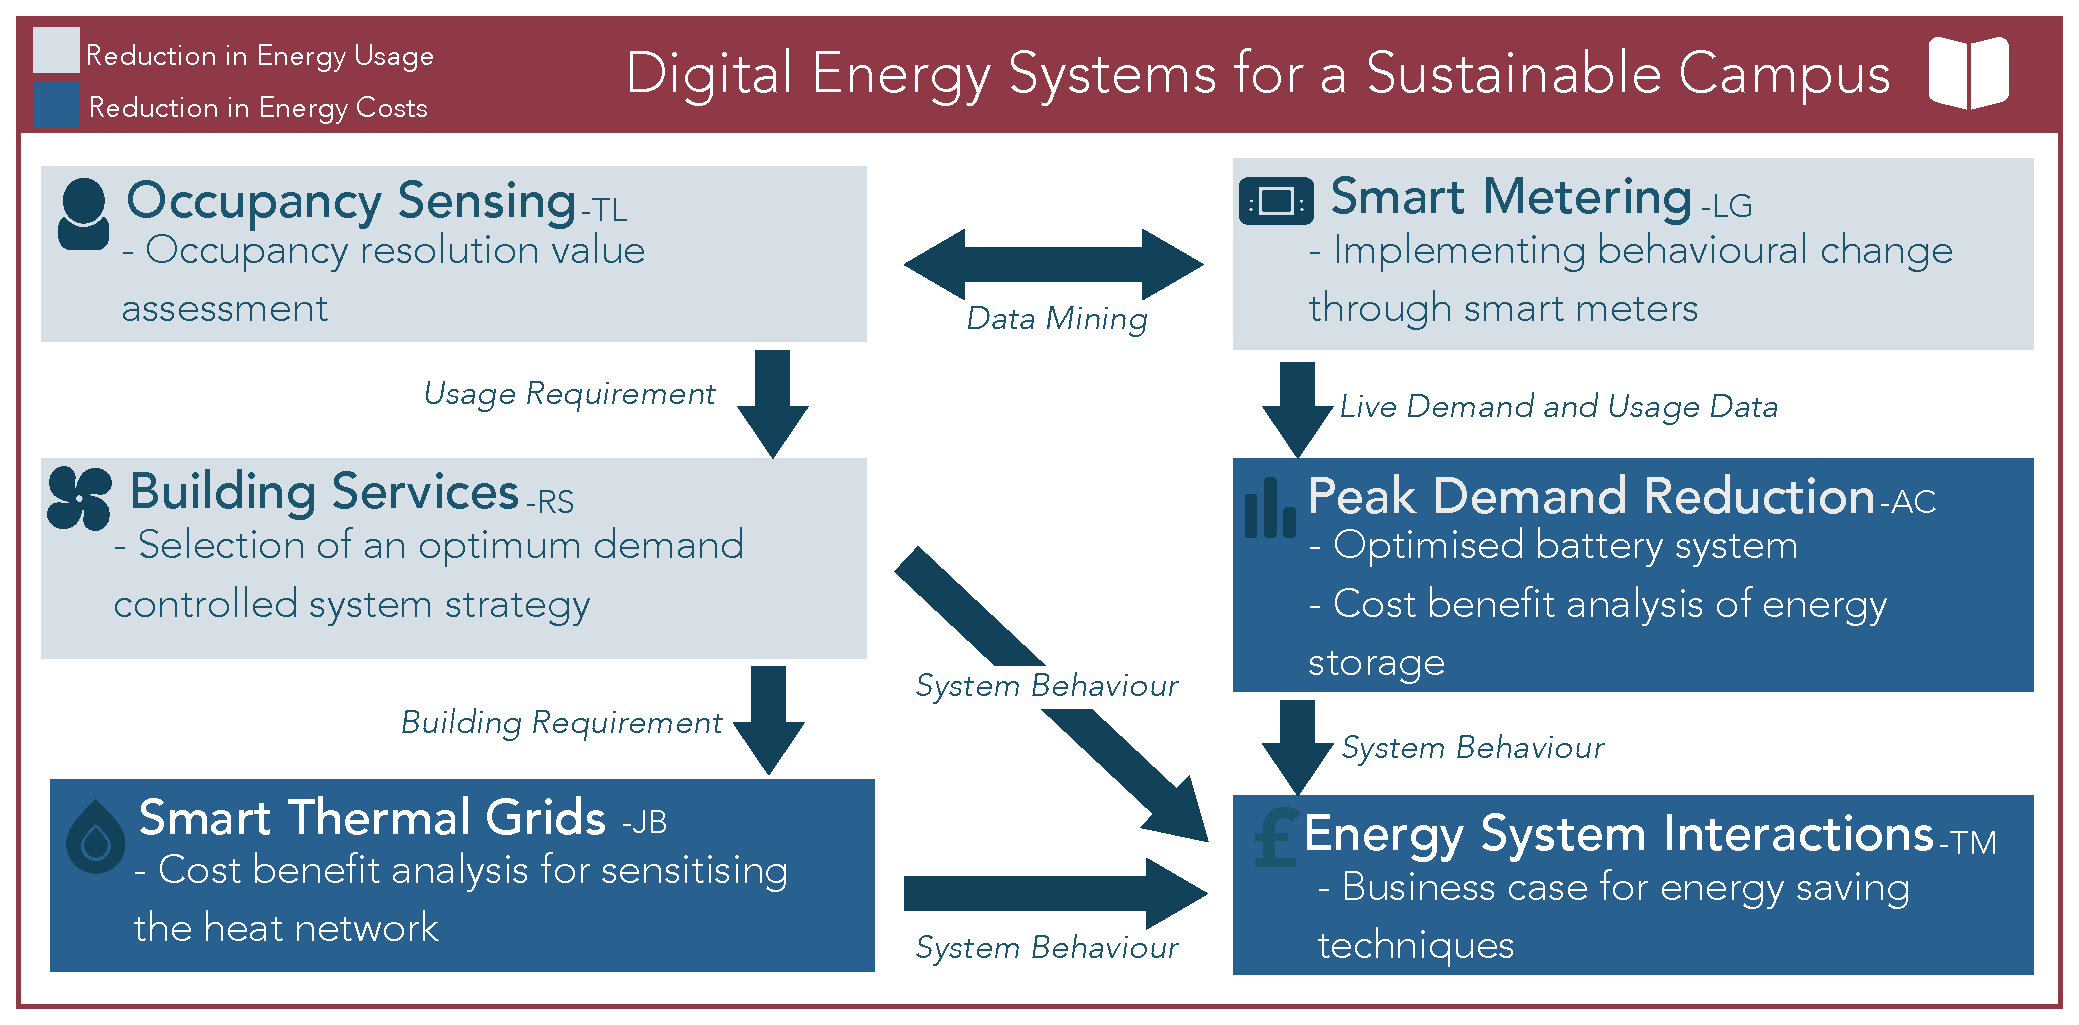
\includegraphics[width=0.75\textwidth]{GroupDiav2.eps}
\caption{Group Design Project Diagram Showing Relationships Between Individual Projects}
\vspace{-20pt}
\label{groupDia}
\end{figure}

\subsection{Individual Project
Introduction}\label{individual-project-introduction}

This project report investigates the feasibility of using energy storage
systems (ESS) to reduce energy charges and increase sustainability for
the University of Bristol. The technology will be implemented in the new
Temple Quarter campus, where this project seeks to provide a a value
incentive for investing in energy storage. Within the project, the
university's energy profile and billing structure are analysed and
simulated, used to define the bespoke energy requirements of the new
campus. A comprehensive technology study of the different ESSs evaluates
the feasibility of various systems, down-selecting the most appropriate
battery for modelling. Through further evaluation of how the selected
battery system would function, a model was designed to simulate battery
system strategies analysing their impact. Finally, to find an optimum
ESS solution, a large range of battery specifications are simulated,
comparing results to find a battery which generates the most value.

The overall outputs of the project for use in the \(5^{th}\) year group
design project are:

\begin{itemize}
\tightlist
\item
  \emph{Cost Based Analysis Business Case}: for investing in battery
  storage technology
\item
  \emph{Energy Profile Tool}: to build and understand the new university
  campus' Demand
\item
  \emph{Optimised Battery System Model}: producing best storage
  solutions based on energy profile tool
\end{itemize}

\subsection{Objectives}\label{objectives}

To achieve the projects outputs, the following detailed objectives were
defined:

\textbf{Literature Review}

\begin{enumerate}
\item Perform a detailed literature review and market analysis of energy storage technologies and research, evaluating using ESS to reduce peak energy demands, highlighting relevant techniques and limitations.
\item Investigate different energy storage solutions for the University's new campus, comparing parameters such as power-ratings, capacity, discharge times and costs to down selecting the best solution.
\end{enumerate}

\textbf{Definition of System Strategies}

\begin{enumerate}[resume]
\item Define battery system strategies, establishing the key performance variables.
\end{enumerate}

\textbf{Modelling and Analysis}

\begin{enumerate}[resume]
\item Analyse the university’s current peak demand charges; understanding the current billing structure and collecting typical energy usage data.  
\item Create a tool to generate demand profile (kW) from half-hourly usage (kWh) data provided defining energy profile of the new campus.
\item Create a model simulating the use of battery strategies to change the energy demand profile of the new campus, comprising of three stages:
\begin{enumerate}
\item A simulation of using the battery system against a current university building, analysing the effect of the system for use as a datum.
\item A simulation of using the battery system in the new university campus
\item An assessment on the optimum battery design to select based on the new campus's energy profile
\end{enumerate}
\end{enumerate}

\textbf{Evaluation}

\begin{enumerate}[resume]
\item Evaluate results of the simulation, concluding on the effectiveness of different battery systems. A cost-based analysis will be used to measure the feasibility of the different energy storage systems for the university comparing the value of the system against current challenges in using the new technology.
\end{enumerate}

\section{Background and Summary of Key Work and
References}\label{background-and-summary-of-key-work-and-references}

The following literature review provides an overview of using Energy
Storage Systems (ESS) to lower energy costs. Using batteries in this
manner is still novel, with a broad range of ESSs and use strategies
available for evaluation; each producing dramatically different results
when placed in different situations. By building a comprehensive
understanding of the technology and new campus situation, an optimised
energy storage system can be found, providing a full understanding of
the value energy storage could bring to the new university campus.

\subsection{Sustainability and Energy Storage
Systems}\label{sustainability-and-energy-storage-systems}

The UK's energy grid uses many methods of providing the power required
to meet the country's demand. This energy comes from both clean (hydro,
wind solar etc.) and dirty (coal, gas etc.) sources. Due to the nature
of most clean technologies, these sources are used to meet the UK's base
load (power usage during off-peak periods) \cite{GBNation22:online}.
Periods of the day when energy usage is higher, (called peak demand)
additional fast-acting dirty sources like combined cycle gas turbines
are switched-on to meet this demand \cite{Reducing94:online}. Peak
demand periods are charged much more significantly, for this reason. An
ESS proposes a new way to level out these peak periods, reducing the
need for fast, responsive dirty technologies. By using energy storage
technologies the University could reduce their emissions by up to
360gCO2 per kWh \cite{Part1Att26:online}, while having the potential to
save a significant amount of money.

\subsection{University Energy Charges}\label{university-energy-charges}

The University of Bristol's infrastructure spans across three sites; the
City Centre, Stoke Bishop and Langford. Across these locations, the
majority of facilities receive separate energy bills, allowing some
granularity in the understanding energy charges originate
from\cite{Jbrentmeet}. The University receives charges bundled together
under four distinct themes \cite{Jbrentmeet}, described below, where
their applicability to energy storage technology is discussed.

\begin{enumerate}
\item \textbf{Unit Charge} - Base cost of energy consumption, making up 58\% of the bill.
\item \textbf{Distribution Use of System (DUoS)} - Including capacity charge and DUoS rate.
\begin{enumerate}
\item \textbf{DUoS Rate} - there are three DUoS rates, Green, Amber and Red \footcite[\label{unitbill}See page 27 of][25.405 p/kWh in Red, against 0.147p/kWh in Green]{SWEB201492:online}, depending on the time of day. Energy costs during Red periods are significantly higher (between 5pm-7pm). For Western Power (University's current supplier), there is a 17000\% increase in price during these periods \footref{unitbill}. Reducing DUoS rate charges is the main method of reducing peak demand charges; an ESS should be used during Red periods and charged during Green periods. These make up ~20\% of the bill \footnote{\label{bill}See Figure \ref{Development-38} in Appendix}.
\item \textbf{Capacity Charge} - this is where the customer sets their maximum demand (kW) level\cite{Deconstr52:online}. This is set above the actual maximum demand of a building, to reduce the risk of breaching this threshold. If breached, the customer incurs substantial penalties, and the supplier increases the threshold for the next billing period. By levelling off peaks in energy demand, the capacity charge threshold can decrease. Capacity charges make up a 4\% of the monthly bill \footref{bill} where the risk surpassing the threshold exceeds any savings seen through implementing an ESS.
\end{enumerate}
\item \textbf{Transmission Network Use of System (TNUoS)} - Three times of the year when the UK's energy demand is greatest, called TRIADs. These dates lie between November and February, separated by at least ten days in each financial year \cite{TriadsWh7:online}. The average max peak demand (kW) across the three TRIADS \cite{TNUoSTra99:online}, is multiplied by a tariff \cite{TNUoScha93:online}; added to the customer's end of year bill. The University has become quite good at forecasting these periods \cite{Jbrentmeet}, making it possible to schedule an ESS to reduce demand during these periods where power supply rate (kW) is crucial. These make up 7\% of the monthly bill \footref{bill}.
\item \textbf{Feed-In Tariff (FIT)} - Based on feeding back energy to the grid. Dependent on the battery system selected, there is potential to increases the value of the ESS by leveraging this charge. This charge is highly complex and frequently changing so will not be evaluated in this project.
\end{enumerate}

\subsection{Current Peak Demand Management
Methods}\label{current-peak-demand-management-methods}

Peak demand reduction is synonymous with peak shaving; the ability to
control energy usage during intervals of high demand, to limit or reduce
demand charges \cite{schneiderRECPS}, \cite{baldorPS}. Traditionally
there are two methods for reducing peak demand for industrial complexes
\cite{schneiderRECPS}. These are:

\textbf{Load Shedding}: This is reducing energy usage, by switching off
certain systems during periods of peak demand \cite{6199851}. An
intelligent scheduling system or a simple forecasting tool can be used
to execute load shedding \cite{Reducing37:online}, where systems are
switched off autonomously or manually. Often load shedding is calculated
daily using a schedule to set a fixed maximum energy limit
\cite{6938948}.

\begin{itemize}
\tightlist
\item
  \emph{Limitations}: Forecasting errors can significantly reduce the
  effectiveness of this system, where reactive methods are often better
  \cite{6938948}. Getting university staff and students to shift their
  usage habits from peak times could be potentially costly
  \cite{Jbrentmeet}, highlighted in experiments conducted by the
  University of Copenhagen \cite{copenmeet}.
\end{itemize}

\textbf{On-site Generation}: Adding off-the-grid capacity to the
consumer \cite{schneiderRECPS}. The University currently uses diesel
generators roughly ten times a year to reduce TRIAD charges; supported
by \cite{shen2016}. Due to the environmental impact of using diesel
generators, an ESS would act as an improved replacement for this method
for reducing TRIAD charges.

\begin{itemize}
\tightlist
\item
  \emph{Limitations}: The University currently has 0.5MW of PhotoVoltaic
  (PV) installed using nearly all available space \cite{Jbrentmeet}.
  These PV's provide only 0.5\% of the total energy demand, meaning the
  use of on-site generation to offset peak demand has a negligible
  effect in flattening the University's demand. Pairing batteries with
  PV as a method of supply levelling appears unfeasible in the context
  of the University.
\end{itemize}

\textbf{University Research}: IODICUS, is a current University project,
looking at reducing energy costs, by improving the amount of sensing
data around the university's usage. This project produced middleware for
an IoT deployment of energy sensors/actuators, and software to explore
the resulting `big data' of the sensors \cite{priestemail}. Although the
project did not evaluate using ESSs, the outcome of improving sensing
data will help to improve the chosen ESS performance.

There are a limited number of commercially available solutions that use
ESSs to reduce peak loads directly. ABB offers energy-storage,
smart-grid, products which perform load levelling at grid level
\cite{abbpeakshave}. These systems are designed primarily for supply
levelling, using forecasting methods and extensive ESSs to offset excess
energy supply produced from renewable energies \cite{5559470}, rather
than focusing on reducing its customer's energy bills. One Cycle Control
have created technologies to regulate peak-load and mitigate peak demand
charges for commercial/industrial facilities using Li-ion batteries
\cite{peakload38:online}. The technologies proved effective at reducing
peak demand charges, but highlight the steep cost of the ESSs reduce the
system's financial feasibility \cite{Demonstr51:online}. Based on there
being no direct commercial solution this report sets to understand the
components required to create an effective energy storage solution for
reducing the university's new campus energy bills.

\subsection{Peak Shaving Systems Literature
Review}\label{peak-shaving-systems-literature-review}

Acknowledging limitations in commercial peak-shaving ESSs, it is crucial
to understand current research in using ESS technology to design an
efficient system. Research is grouped, highlighting each section's
significance and relevance to the development of the model.

\subsubsection{Forecasting and the Use of ESS in Load
Shifting}\label{forecasting-and-the-use-of-ess-in-load-shifting}

Using energy price forecasts, an ESS can be switched on to shift energy
costs; purchasing energy at a cheaper rate, using this energy during
peak times. \cite{7555795} ran simulations to test NaS, Li-ion and Flow
batteries, for an Italian commercial plant, failed to find viable return
on investment (ROI)\cite{7555795}.\cite{5590194} used real hourly spot
prices to decide the best times to turn on and off Vanadium Redox
Batteries (VRB) and Polysulfide Bromide Batteries (PSB). Through
sequential quadratic programming (SQP), battery sizes were optimised,
finding PSB's had a business case for load shifting. These two
conflicting results were due to the sensitivity in energy pricing. An
independent investigation of this technique with the University, may
prove feasible. \cite{Bennett2015122} added a real-time operator to
create an intelligent scheduling system for home prediction. This system
significantly improved the state of charge of the battery, freeing more
energy for use in reducing peaks, highlighting that forecasts combined
with real-time information can increase the performance of the system
further. Modelling development will research:

\begin{itemize}
\tightlist
\item
  the implications of battery health on the lifetime value of the
  battery, for the battery selected
\item
  increasing granularity in the University's usage data will to
  incorportate a real-time operator
\end{itemize}

\subsubsection{Supply Levelling}\label{supply-levelling}

Supply levelling is the most common use for ESS \cite{iearoadmapes},
using large batteries to reduce power fluctuations brought by the use of
renewable technologies \cite{7324861}, \cite{7564619}. Supply levelling
works by storing excess supply, reducing peaks in the grid rather than
in demand. \cite{Allik20161116} looked at improving supply for a
residential home. Shiftable water heating was identified to account for
50\% of household electricity use, so was used as the primary storage
device. Excess load from wind turbines was used to heat water in excess
supply periods bypassing an inverter improved energy losses
\cite{Leadbetter2012685}. Minimising conversion through inverters makes
a large difference in the efficiency of the system. Supply levelling
will not be addressed in this model due to the University's PV's
contributing to only 0.5\% of its supply \autocite{Jbrentmeet}.

\subsubsection{Battery Sizing and Financial
Modelling}\label{battery-sizing-and-financial-modelling}

There are numerous studies, analysing the business cases for ESSs.
\cite{7555795} and \cite{7555793} model the use ESSs broadly, to reduce
the cost of all energy charges, revealing that the ROI is unlikely to be
feasible beyond 2020. Papers including \cite{1300158} and \cite{6175723}
evaluated financial models for particular case studies, showing that
bespoke solutions achieved greater peak shaving reductions than returns
promised by current generic products \cite{abbpeakshave}.
\cite{7555795}, \cite{7555793}, \cite{1300158}, \cite{6175723} and
\cite{20164002874437} all present a strong arguments that a bespoke
solution for the University will provide a better business case for ESS
than generic commercial technology.

Investigating the benefits of a decentralised system, reducing peaks on
a small scale rather than using one large central ESS, \cite{6604477}
analysed both peak shaving and battery longevity for a large data
centre. Through both experimentation and modelling, \cite{6604477}
showed that when regarding the batteries lifespan, the ability to
regulate load through a series of batteries can be more favourable than
a centralised system. Research conducted by \cite{6348200} and
\cite{Demonstr51:online} also both support using a decentralised system.

\cite{20160601898032}, \cite{Levron201280} and \cite{5371839} show
methods ways of optimising battery configurations. \cite{5371839}, used
a non-numeric modelling method, focusing on ultra-capacitors to find the
optimal ESS. The results emphasised the constraint of storage capacity,
showing an exponential decrease in value gained after a particular size
of ESS. Finding the required battery size and power for the new campus
will be the primary focus of this project's model. \cite{Levron201280}
created an analytical model, using energy bands to regulate peak load,
giving an optimum storage size for a given system; this was a
straightforward and efficient method of modelling battery usage. The
model will incorporate:

\begin{itemize}
\tightlist
\item
  An adaption of \cite{20160601898032} modelling technique to find the
  optimal configuration of the ESS
\item
  An assessment a decentralised battery system, focusing primarily on
  lab space
\end{itemize}

\subsection{Comparison of Energy Storage
Systems}\label{comparison-of-energy-storage-systems}

The selected ESS will govern the cost and feasibility of a peak shaving
system. An ESS converts electrical energy into a form stored for later
use \cite{Chen2009291}. Electrochemical batteries characterise low
maintenance, high round-trip efficiency, long cycle lives and high
energy density's; arguably being the most appropriate technology for
peak shaving \cite{liao2016a}, \cite{Dunn928}. Batteries, therefore,
have been chosen as the main focus for this study. The various storage
methods can be characterised for different uses summaries below:

\begin{itemize}
\tightlist
\item
  \textbf{Energy Management:} for large scale storage, typically used by
  power plants for load levelling and ramping/load following.

  \begin{itemize}
  \tightlist
  \item
    Pumped Hydroelectric Storage (PHS), Compressed Air Energy Storage
    (CAES) and Cryogenic Energy Storage (CES) are the conventional
    technologies for high generation above 100MW. All these methods are
    on a scale too large to be considered for this project.
  \item
    Large-scale batteries, flow batteries, fuel cells, solar fuels, CES
    and Thermal Energy Storage (TES) are suitable for medium-scale
    energy management with capacities of 10 -- 100 MW. These
    technologies are too large and their frequency response is too slow
    for this application.
  \end{itemize}
\item
  \textbf{Power quality:} fast response times improve power quality
  allowing techniques such as the instantaneous voltage drop, flicker
  mitigation and short duration uninterrupted power supply

  \begin{itemize}
  \tightlist
  \item
    Flywheels, Batteries, Superconducting Magnetic Energy Storages
    (SMES), capacitors and ultra-capacitors have millisecond response
    time lower for storage sizes less than 1 MW - suitable in addition
    to large scale battery.
  \end{itemize}
\item
  \textbf{Bridging power:} Relatively fast response (\textless{} 1 s)
  but also have relatively long discharge time (hours). The typical
  power rating for these types of applications is about 100 kW -- 10 MW.

  \begin{itemize}
  \tightlist
  \item
    Batteries, flow batteries \cite{flowbatstan}, fuel cells and
    Metal-Air Cells\cite{Chen2009291}, \cite{batuni}. These are the most
    appropriate ESS type for application.
  \end{itemize}
\end{itemize}

By removing energy storage methods that would not be appropriate for the
system a table was created
\footnote{See table \ref{battabs}, in the Appendices} comparing ESSs.
Batteries along with capacitors provide the response time
\cite{Choudar201521} and efficiencies required to make the system
justifiable, where only rechargeable batteries were compared.

\subsection{Battery Selection - Tesla Powerpack
2}\label{battery-selection---tesla-powerpack-2}

Due to the maturity of the technology, the fast frequency response in
delivering power, Li-ion batteries were down-selected as the most viable
option for achieving the project's aims. EOS and BYD and Tesla are
currently the only companies that supply Li-ion batteries of an
appropriate size. Due readiness in information around performance and
price, the Tesla Powerpack 2 was chosen for this model, to improve the
validity of results.

\section{Battery Storage Technology Key Advantages and
Challenges}\label{battery-storage-technology-key-advantages-and-challenges}

Table \ref{AdChalltab} identifies the key values and challenges of using
Li-ion technology. Overcoming challenges with high severity by
developing a comprehensive understanding of their effects is the focus
of the model developed in this project. This is necessary to create an
effective cost based analysis of using a Li-ion energy storage system.
To create strong arguments to how the system will overcome these
challenges, assumptions used overcome these issues are discussed in this
section.

\begin{table}[H]
\vspace{-10pt}
\caption{Showing the Advantages and Challenges of Using Energy Storage}
\vspace{-5pt}
\centering
\includegraphics[trim = 0 0 0 0, clip, width=0.9\textwidth]{AdvantChallTab.pdf}
\label{AdChalltab}
\vspace{-15pt}
\end{table}

\subsection{Battery Economics}\label{battery-economics}

The primary objective of this project is to create a cost-based analysis
business case for using a battery system giving a valid prediction of
the value an ESS could generate. There are three ways the model will
assess the value of the storage system; \emph{net present value},
\emph{pay-back period} and \emph{total-savings}. Each of these results
will be compared, crediting their merits and pitfalls, to give a full
understanding of the battery's value.

\subsubsection{Net Present Value}\label{net-present-value}

Net Present Value (NPV) describes the difference between the current
value of cash inflows and outflows \cite{NetPrese35:online}. NPV is used
in capital budgeting to analyse the profitability of an investment over
the long-term. Batteries are a significant upfront investment, seeing
little financial value for many years. As a consequence, purchasing the
battery through finance is likely, adding an interest rate to the cost
of the battery. Battery degradation and inflation are also factors,
increase the discount rate required to correctly value financial
performance over time.

The Internal Return Rate (IRR) is a method for finding the maximum
discount rate before that an asset generates a negative NPV. This is
found by setting the net present value to 0 and calculating the return
rate. Equation \ref{eq:IRR}, defines the secant numerical method used
for calculating the IRR.

\begin{align}
r_{ n+1 }=r_{ n }-{ NPV }_{ n }\cdot \left( \frac { r_{ n }-r_{ n-1 } }{ { NPV }_{ n }-{ NPV }_{ n-1 } }  \right)
\label{eq:IRR}
\end{align}

Where \(r_{ n }\) defines the \(n^{th}\) approximation of the IRR
\cite{xxxdvi44:online}.

Using Equation \ref{eq:IRR} the maximum discount rate can be found using
batteries at the extremities of the results (lowest and highest
performers). If the IRR is found to be too low, the battery strategies
will need revising otherwise it can be concluded that it is not feasible
to invest in an ESS
\footcite[An IRR below 5\% is considered unfeasible, although unquantified benefits may be present][]{diorio2015economic}.\\
Total savings is the measure of NPV when the discount rate is set to
zero; providing a clear understanding of the cash flow which the system
generates.

\subsubsection{Payback Period}\label{payback-period}

\begin{wrapfigure}{r}{0.35\textwidth}
  \begin{center}
    \vspace{-45pt}
 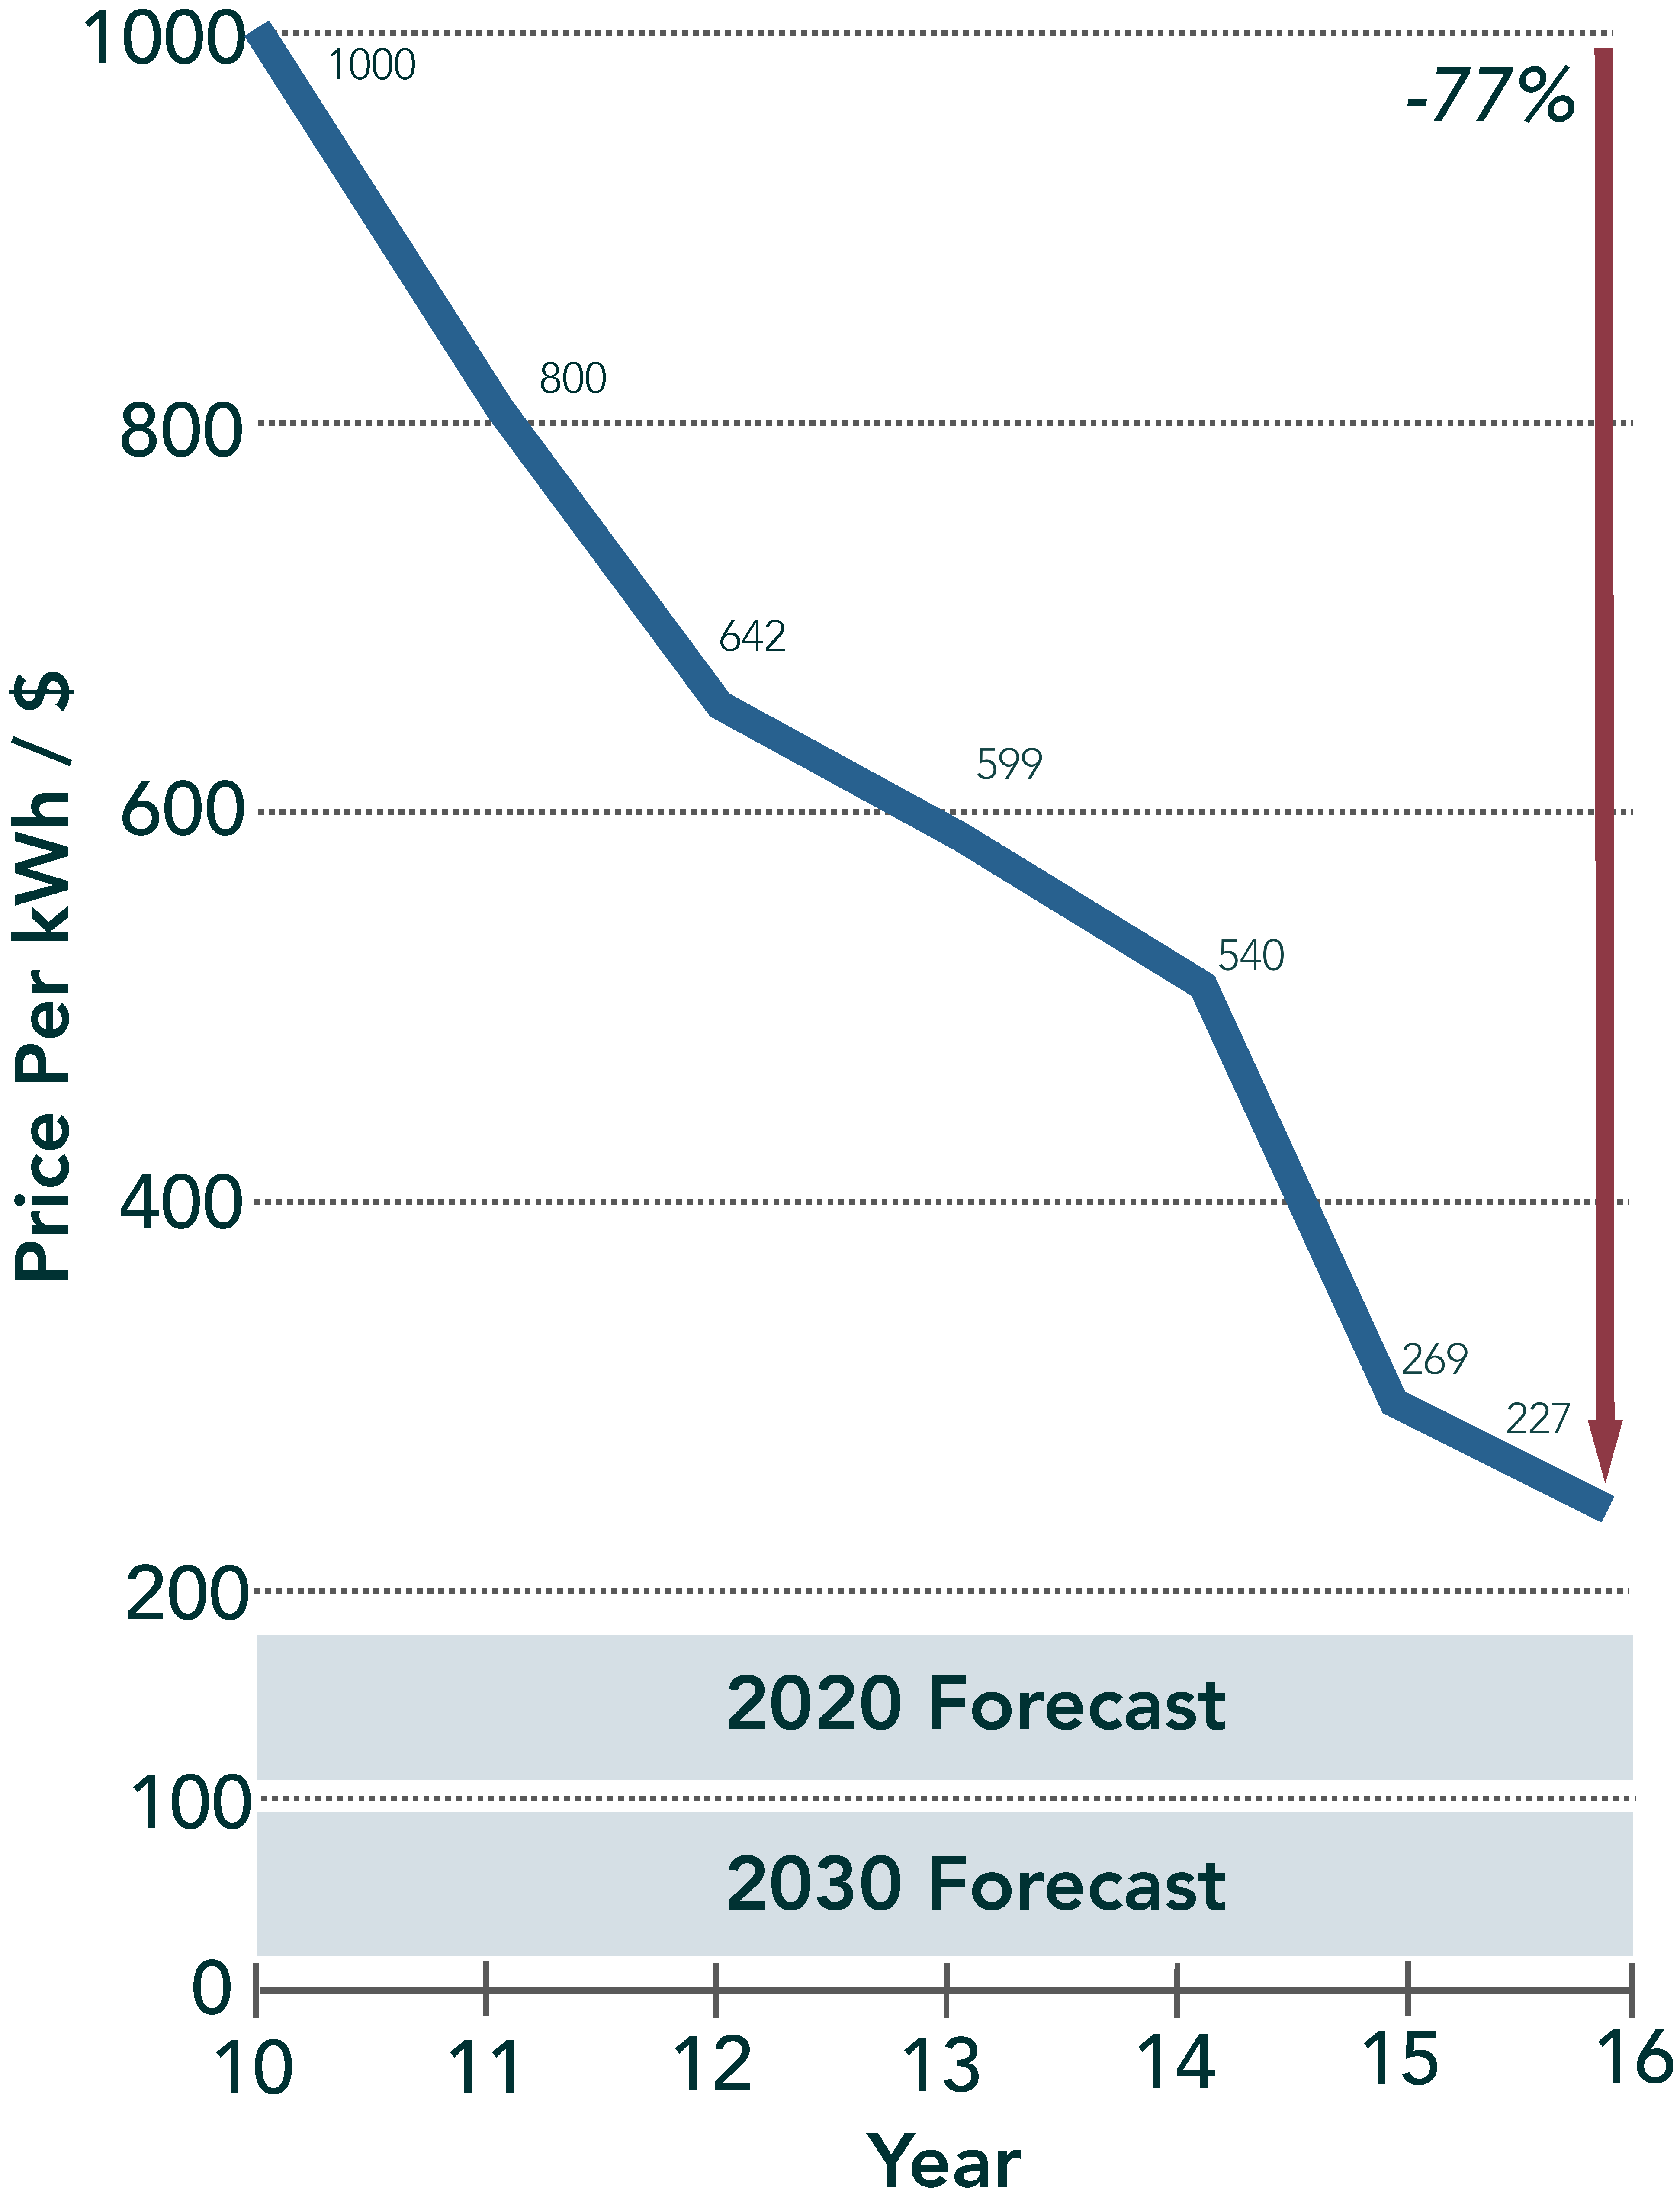
\includegraphics[trim = 0 0 0 0, clip, width=0.34\textwidth]{BatPrice.eps}
  \end{center}
  \vspace{-5pt}
  \caption{Plot of Li-ion Battery Prices 2010-2016 \cite{mckBat}}
  \vspace{-30pt}
  \label{mckBatPrice}
\end{wrapfigure}

The Payback Period (PBP) is the time for project savings to equal or
exceed the cost of the investment \cite{diorio2015economic}. This metric
is used to measure risk. Minimising the payback period diminishes many
high severity challenges of the battery, reducing the likelihood of
energy billing change and the likelihood of the battery failing. The
Tesla Power-pack 2 has 10 years warranty, reducing the risk of
additional costs to replacement/repair the battery before it becomes
profitable. As the battery will be viewed first as a financial
investment by the University, having a short enough payback period will
be essential to proving the battery systems viability.

\subsection{Li-ion Battery Costing}\label{li-ion-battery-costing}

Over the last decade, Li-ion technology has advanced significantly,
partly due to the rise in electric vehicles, slashing the price while
improving efficiencies and energy densities. Figure \ref{mckBatPrice}
shows the trend in prices for the last six years and the predictions for
the next 15. Between 2010 to 2016, battery pack prices fell
\textasciitilde{}77\% from \$1,000/kWh to \$227/kWh. Current projections
put the price of Li-ion battery pack prices below \$190/kWh by the end
of the decade, corresponding with the construction of the new campus, an
further 16\% reduction, consequently the feasibility of investing in the
technology will continue to increase.

Data readily available on the Powerpacks's based on the battery's
capacity (kWh) and maximum power (kW) \cite{Powerpac95:online}. This
makes it possible to evaluate the optimum specification of battery for
an energy profile. Unit costs start at £51,940 and scale infinitely.
After purchasing the product, installation is the next largest cost to
consider. The Powerpack comes almost as plug and play, including an
inbuilt inverter simplifying the process extensively. The cost to
install will be significantly greater when retrofitting to existing
infrastructure as it is assumed a suitable foundations are necessary due
for the battery fully operational in a university environment. In the
case of the new campus, it is assumed that there are little additional
costs in installing the battery system due to installation requirements,
placed on the site's design.

Maintenance/operations costs are another factor to consider. The
Powerpack uses a health checking system, requiring little training to
monitor the battery. It seems likely that the University can use a
member of the Estates team monitor the battery infrequently. Section
\ref{payback-period}, discussed the Powerpack ten-year warranty,
eliminating any costs in the first 10 years. For these reasons
maintenance/operations are assumed negligible.

By using today's battery prices, it is assumed the battery's cost will
be under-estimated compared to when it will be installed in the new
campus. This will reduce the uncertainty around the costing assumptions
made.

\subsection{Battery Lifetime Assessment - Understanding Battery
Degradation}\label{battery-lifetime-assessment---understanding-battery-degradation}

\begin{wrapfigure}{r}{0.4\textwidth}
  \begin{center}
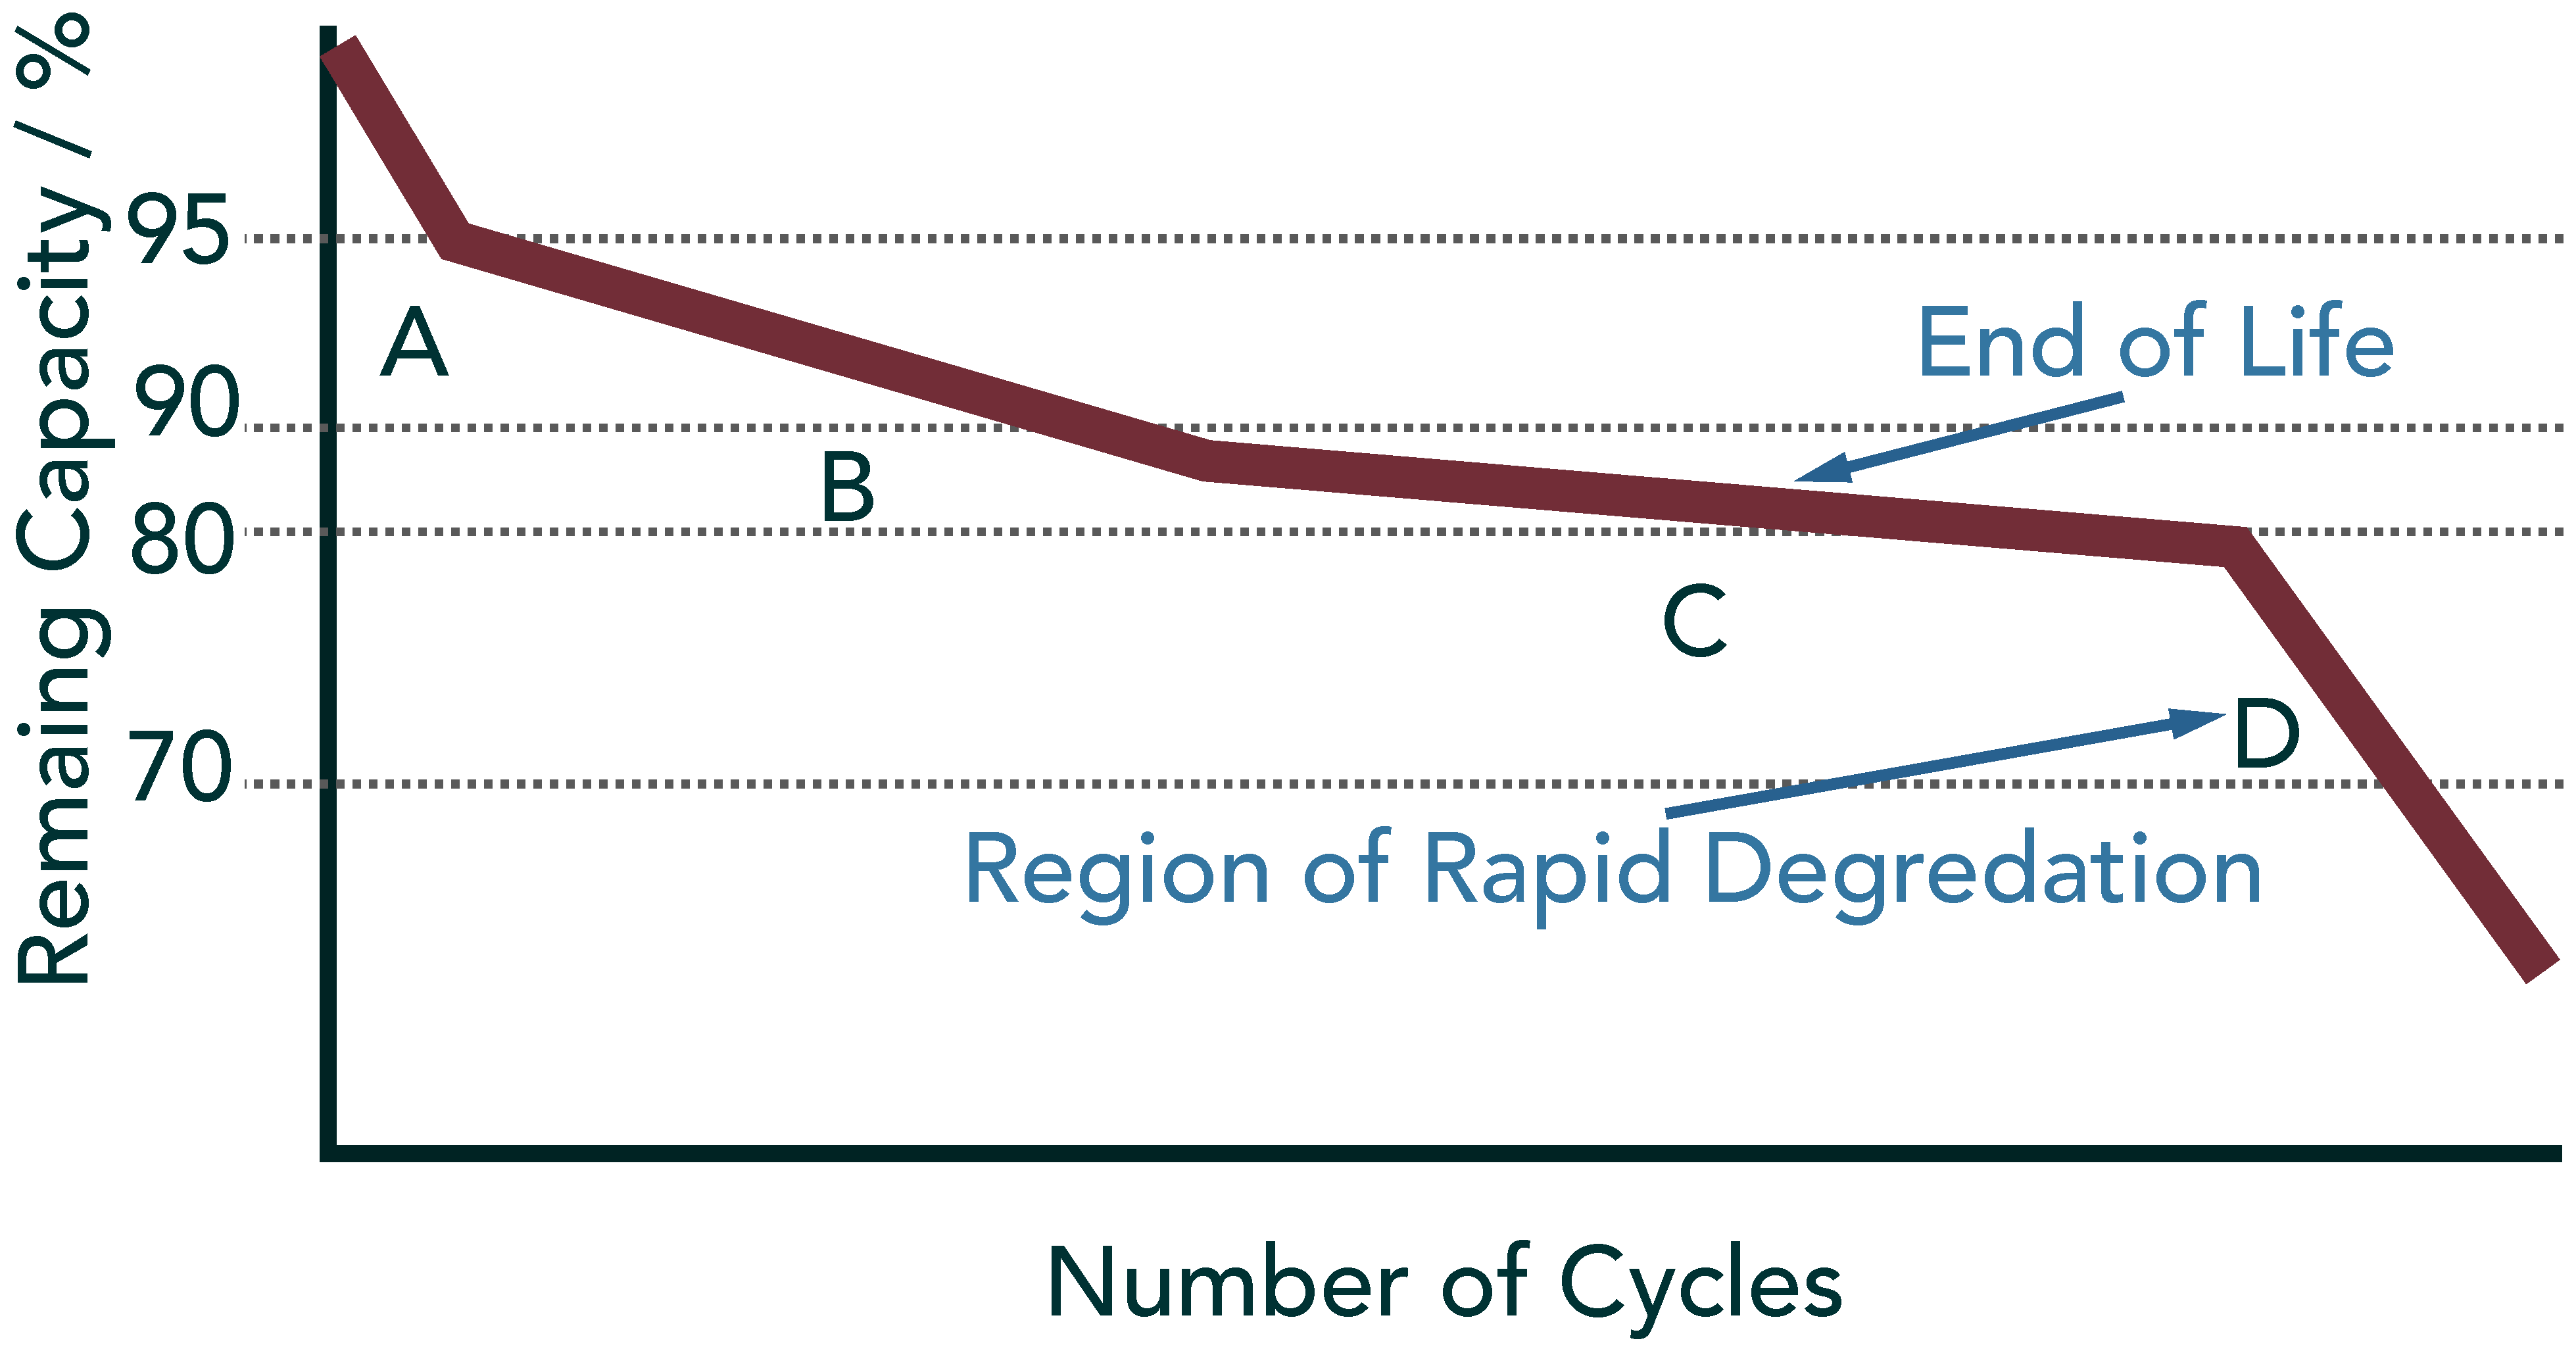
\includegraphics[trim = 0 0 0 0, clip, width=0.39\textwidth]{CapCycle.eps}
  \end{center}
    \vspace{-5pt}
\caption{Plot of the General Relationship Between Battery Capacity and Cycle Number Extracted From \cite{spotnitz2003simulation} }
  \vspace{-20pt}
  \label{batCapGen}
\end{wrapfigure}

Sections \ref{forecasting-and-the-use-of-ess-in-load-shifting} and
\ref{battery-sizing-and-financial-modelling}, highlighted the importance
of battery health in increasing the longterm value of an ESS. By
operating the battery in a way that considers its longevity, further
value can be generated. To correctly model how the Li-ion batteries
degrade over time, the following section explains the different
parameters which effect on battery health discussing how they should be
regarded in the model.

Figure \ref{batCapGen} shows the typical capacity degradation profile of
a Li-ion battery. After the battery degrades below 80\% (C) of it is
original capacity, it is regarded to be in its end of life phase
\cite{REIEC61465:online}. After this point, degradation becomes more
rapid and unpredictable \cite{spotnitz2003simulation}. There is still
potential for more energy to be delivered beyond this point
\cite{Renaultt62:online}, however, for the model to remain
representative, after the battery's health reaches 80\%, the battery
should be regarded as dead.

The following list of parameters, gives a brief overview of these effect
battery degradation, highlighting how they are regarded in the model

\subsubsection{Temperature}\label{temperature}

By running the battery at a temperature too hot or too cold, increases a
batteries rate of degradation significantly \cite{rong2006analytical}.
The Tesla Powerpack incorporates an internal liquid cooling and heating
system which allows for pinpoint temperature control. A dual coolant and
refrigerant loop system minimises the effects of temperature
degradation, climates providing better efficiency than traditional HVAC
systems. \cite{Powerpac95:online}. Due to safety reason, it is recommend
that the battery is installed outside, making the battery susceptible to
climate. England experiences a mild climate all year round, spending
most of it is time between 3\degree C and 22\degree C
\cite{WeatherA0:online}. These cooler temperatures favour the battery's
performance. For both these reasons, the model will assume temperatures
effect on degradation is negligible.

\subsubsection{Depth of Discharge (DoD)}\label{depth-of-discharge-dod}

\begin{wrapfigure}{r}{0.5\textwidth}
\vspace{-40pt}
  \begin{center}
\includegraphics[trim = 0 0 0 0, clip, width=0.49\textwidth]{dodplot22.eps}
  \end{center}
    \vspace{-5pt}
  \caption{Plot of Depth of Discharge vs Rated Capacity, Interpolated From \cite{BatteryL10:online}}
  \label{dodLog}
  \vspace{-10pt}
\end{wrapfigure}

Depth of discharge is related to the number of active chemicals
transformed with each charge/ discharge cycle
\footnote{See Figure \ref{BatteryImage}, for a detailed description of battery cycling}.
Figure \ref{dodLog} shows experimental results of the effect of DOD on
Lead-Acid batteries capacity, holds true for Li-ion
\cite{BatteryL10:online}. At the rated cycle life of 5000, is was
assumed a 70\% DOD was used to test the battery lifespan
\cite{Teslawil27:online}. This value was scaled accordingly. By
restricting the possible DoD cycle life of the battery can be
dramatically improved. It is common practice to select cells with more
capacity than required. The battery's average depth of discharge over
its lifetime should be recorded and used as a metric for the validity of
the selected batteries expected lifetime.

\subsubsection{Usage}\label{usage}

\begin{wrapfigure}{r}{0.5\textwidth}
\vspace{-40pt}
  \begin{center}
\includegraphics[trim = 0 0 10 0, clip, width=0.49\textwidth]{dischargetime.pdf}
\vspace{-5pt}
  \caption{Plot of the Relationship Between Discharge Time and Rated Capacity, Interpolated from \cite{Effectso69:online}}
    \end{center}
  \label{disRate}
  \vspace{-20pt}
\end{wrapfigure}

\emph{Over Depletion}: Fully depleting a battery for extended periods
can have detrimental effects on capacity. It is common for battery
management systems (BMS), particularly in consumer electronics to power
devices off above zero; negating some of the effects of depleted storage
levels \cite{Prematur82:online}. The model should prevent the battery
from being depleted below 10\% to offset this effect.

\emph{Discharge Time}: When discharging batteries quickly, the effective
capacity of the cell can be reduced \cite{BatteryP62:online}. The
Peukert Equation is a method used to characterise cell behaviour with
regards to capacity offset, when depleting the battery at high discharge
rates. It is unclear what the Powerpack's Peurket number is, but it can
be assumed to be between 1-1.02, where 1 is perceived as the battery
performing well. \cite{omar2012rechargeable}, \cite{omar2013peukert}
\footnote{Li-ion's low Peurket number is another strong supporting factor why using Li-ion is well suited reducing peak demand where there may be instantaneous high levels in demand}.
The low Peurket number means discharge rate up to the rated power, has
little effect on the battery's perceived capacity. Rate of discharge
also effect the batteries
lifetime\cite{BatteryL10:online},\cite{Effectso69:online}. Using the
experimental trend shown in Figure \ref{disRate}, an equation for the
effect of speed of depletion can be used to validate the effect of
average discharge time. This parameter should be recorded by the model.

\subsubsection{Charging}\label{charging}

\begin{wrapfigure}{r}{0.4\textwidth}
\vspace{-55pt}
  \begin{center}
\includegraphics[trim = 0 0 0 0, clip, width=0.4\textwidth]{SoCgraph.png}
  \end{center}
  \vspace{-5pt}
\caption{Relationship Between State of Charge and Cycle Life \cite{xu2016modeling}}
  \label{SoCgraph}
  \vspace{-20pt}
\end{wrapfigure}

\emph{Charging Level}: The cycle life of a battery can be increased by
reducing the cut-off voltage of the battery. Battery voltage will be
fixed at either high voltage three phase or at single phase 240V, where
current drawn into the battery will vary. Decreasing the battery's
voltage will extend its life (partial charging) \cite{Choi2002130}
\footnote{ See Figure \ref{capVol} in the Appendix, showing the relationship of cell capacity and charge voltage, where  a dramatic decrease in cell performance for cells charged to higher levels is visible}.
By charging the battery too its' full capacity, or overcharging, the
battery capacity will degrade quicker, becoming unstable. Cell chemistry
causes pressure to rise, increasing temperature inside the cell, further
reducing in the battery's capacity. The cell also has a lower thermal
runaway temperature and will vent its temperature quicker than one that
is partially charged. Consequently, Li-ion batteries are safer at a
lower charge \cite{Charging53:online}. Due to these two issues, the
battery should stop charging before reaching this threshold.

\emph{Charging Rate}: Similar to discharge time, a reduction in battery
capacity occurs at high discharge rates; due to the transformation of
the active chemicals inside the cell being unable to keep pace with the
current drawn, reducing cell capacity \cite{BatteryL10:online}. The
model should maximise the charge time of the battery, to reduce this
effect.

Figure \ref{SoCgraph} shows testing conducted on Li-ion cells combining
the ideas found from battery charging and depth of discharge to increase
the lifetime of the battery. Using this result, a charging range can be
selected which optimises the payback period of the battery against the
battery's lifetime.

\section{Battery Model Definition}\label{battery-model-definition}

Through understanding the key design parameters for reducing the impact
of challenges set in section
\ref{battery-storage-technology-key-advantages-and-challenges}, a viable
model of the battery system was defined. Data was obtained for Senate
House (a 7-storey University office/study building). This was used to
create a characteristic demand and usage profile for Senate; then
manipulated to create a representative energy profile for the New
Campus. This section will define how the model was created, discussing
the methodology and any assumptions made. Figure \ref{SystemLogic1}
describes an overview of the primary inputs, processes and outputs of
the model.

\begin{figure}[H]
 \centering
   \vspace{-7pt}
 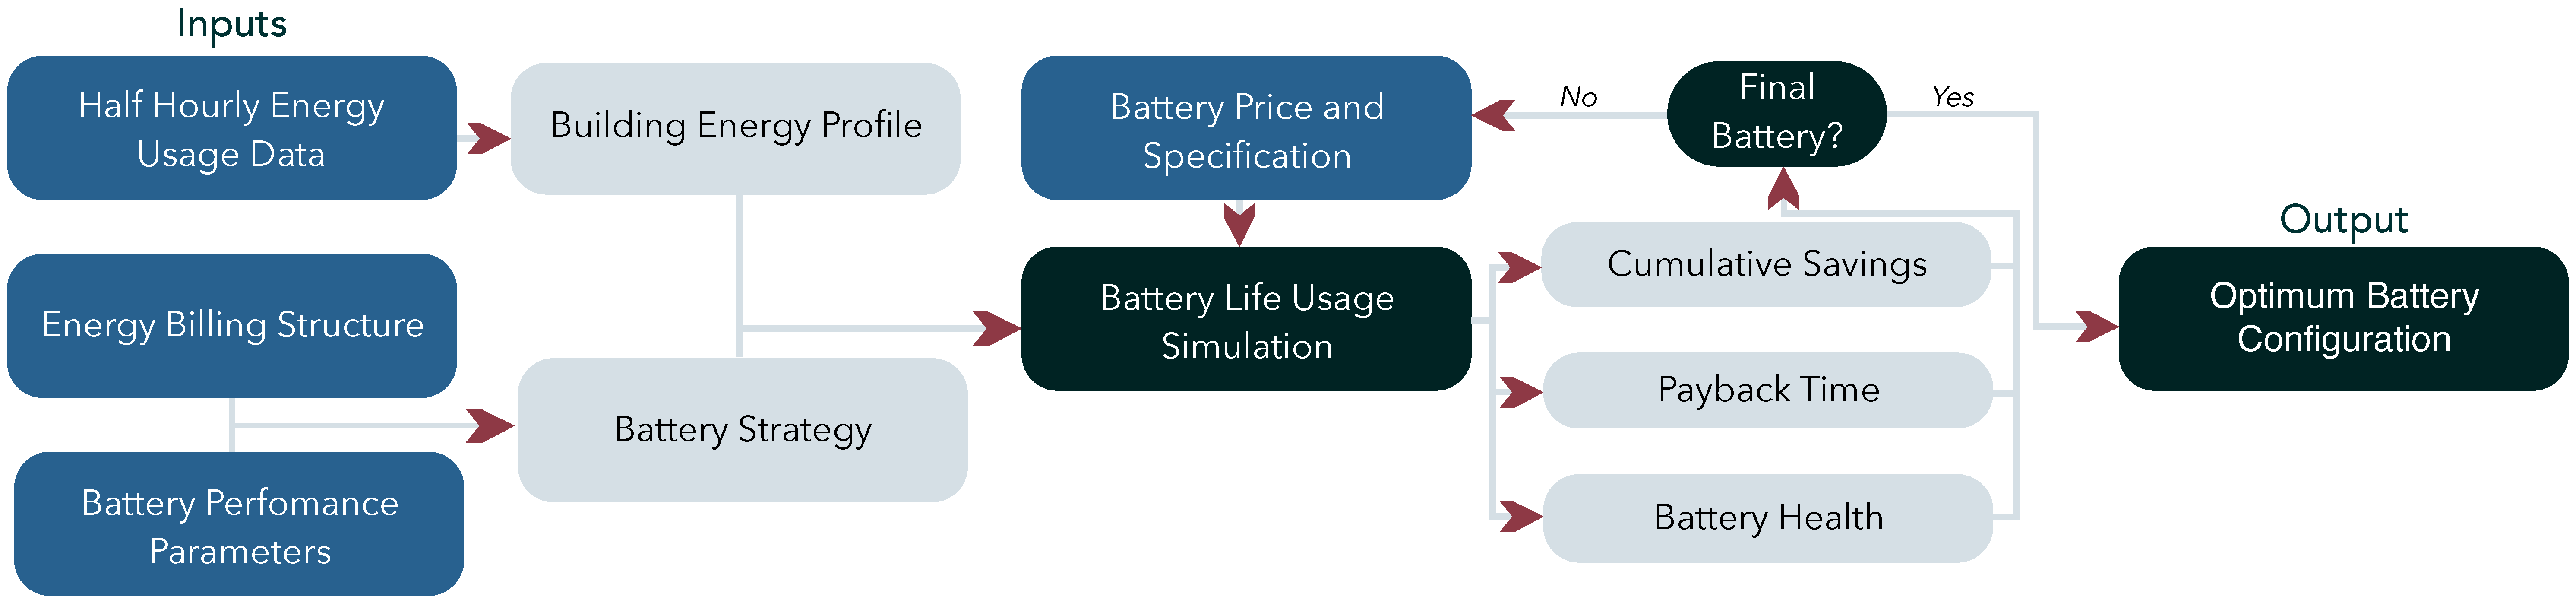
\includegraphics[trim = 0 0 0 0, clip, width=0.9\textwidth]{SystemLogic1.eps}
  \vspace{-10pt}
 \caption{Diagram Showing Key Inputs, Processes and Outputs of Model}
 \label{SystemLogic1}
 \vspace{-30pt}
 \end{figure}

\subsection{Model Development
Requirements}\label{model-development-requirements}

A distinct set of modelling requirements were essential to ensure that a
functional model was created which corresponded to the project's
objectives. By building a flexible, simple model, any unnecessary
complexity was removed; sparing both time and computational expense. A
robust set of requirements also provided a basis for assessing the
completeness of work. The following section defines these requirements.

\subsubsection{Zero-Dimensional vs.~Three-Dimensional
Modelling}\label{zero-dimensional-vs.three-dimensional-modelling}

The zero-dimensional modelling approach is a technique used in the
development cycle of a product, typically in the early stages.
Zero-dimensional models are used to understand general performance of a
system \autocite{ZeroDMod80:online}. Instead three-dimensional models
are implemented when detailed analysis is needed. The system dynamics of
a zero-dimensional model are a function of the time while a
three-dimensional model is a function of the time and space. For this
reason, a zero-dimensional models are simpler and faster at generating
solutions; enabling a much large number of simulations to be run. As
multiple battery systems and strategies are being evaluated,
zero-dimensional modelling method was used.

\subsubsection{Code Optimisation and Ease of
Development}\label{code-optimisation-and-ease-of-development}

A time-based iterative modelling method, based on a zero-dimensional
approach, was selected to model a large variety of different battery
specifications. Running the simulation through time requires performing
calculations on large matrices. The model should be optimised for
performance to minimise running times; helping improve the model
performance and reduce data collection time, allowing for a greater
amount of different battery specifications to be modelled
\footnote{See section \ref{input-parameters-and-multi-battery-simulation} the methods used to create optimised code}.
It is essential that the model remains structured to allow for expansion
as the project progresses. A function based approach must be taken
throughout the development process to allow the model reach to its
expected size and complexity. Without functions, structure will be poor
increasing the difficulty in further develop and debugging.

\subsubsection{User Interface}\label{user-interface}

There is a strong likelihood of using this model for next year's group
design project. The modelling functions outlined in the project's
outputs, should operate independently from each other, working with a
broad range of data. Being able to manipulate the model easily will mean
others will be able to use the tools developed, making the model much
more useful. The model, consequently, must allow for a range of inputs,
which should be easily configurable. Design the model in this way, will
also simplify data collection reduce the risk of introducing a systemic
error, associated with the user entering incorrect inputs or false
logic. Dates and times of the energy usage data inputted in the model
will have a large effect on the results. It is important therefore that
the model can read data files and use their dates, to create accurate
runtime usage data. The data outputted by the model must be clear and
easy to interpreted by any user, with minimal post-processing; this will
improve the model's ability to be a design tool.

\subsection{Creation of Senate House Billing
Model}\label{creation-of-senate-house-billing-model}

In order to validate the results of the model before testing on the new
campus, the model was developed for use Senate House.

\begin{wrapfigure}{r}{0.5\textwidth}
  \begin{center}
    \vspace{-5pt}
 \includegraphics[trim = 0 0 110 0, clip, width=0.49\textwidth]{wkendwkday.eps}
  \end{center}
  \vspace{-10pt}
  \caption{Plot of Mean Senate House Weekday and Weekend Usage, and Difference in Unit Charge Rates}
  \vspace{-20pt}
  \label{wkendwkday}
\end{wrapfigure}

Data for Senate House, was provided; describing half-hourly usage
between 10/08/2014 and 10/08/2015. A bill was also provided for a months
energy usage at the Victoria rooms
\footnote{A Bristol University building used for lecturing, offices and teaching classes, see Figure \{Development-38}
for the Bill provided\}. A meeting with John Brenton \cite{Jbrentmeet}
clarified that billing profiles for both buildings were identical. In
order to gauge the size and power requirements of a battery system for
Senate House, a minute by minute energy profile was required.
Corresponding this energy profile with a bill identified how energy
consumption correlated with the cost, allowing quick sensitivity
calculations to select strategies likely to would have the greatest
impact.

Using this data, plots were used to visualise key trends in energy
consumption, such as the variation of used based on time of day and
period in the year. It was clear that the was a major difference between
energy demand during the weekend and during the week, shown in
\ref{wkendwkday}, where total energy consumption was found to be three
times greater over weekdays than the weekend. It was vital all these
trends were replicated when the usage file was manipulated.

\subsubsection{Representative Bill
Creation}\label{representative-bill-creation}

Section \ref{university-energy-charges} described the components of the
energy bill. It's clear that Red rate charges are a significant charge
which an ESS can target, incorporating \textasciitilde{}20\% of the
bill. To highlight the significance of the Red rate charge, Figure
\ref{wkendwkday} shows the difference in DUoS rates. A preliminary model
was designed to target Red rate charges only through load shifting.
Using Senate's half-hourly data, each DUoS rate charges and unit charges
was calculated. The energy profile was scanned to find which day the
bill began, assigning each day as a weekends or weekday, crucial as Red
rate charges aren't applicable on weekends. By creating a counter that
looped through each half hour period, logic was be applied to categorise
each half hour period into their respective unit rate. Total units
consumed in Red, Amber and Green periods were found, where simple
calculations revealed the the effect of load shifting could have. This
crude model captured 79\% of the monthly energy bill charges.

\subsection{Representative Demand
Profile}\label{representative-demand-profile}

To simulate how a battery performs, power and capacity must be
considered. Applying too much load on a battery can severely reduce the
batteries cycle life, discussed in section
\ref{battery-lifetime-assessment---understanding-battery-degradation}.
Due to the lack of available demand data for the University, assumptions
were made to generate a valid demand profile based on the original
half-hourly usage profile.

First, the usage data was broken down into a minute by minute
representation. Through using linear interpolation, an identical looking
graph of the original data was created, containing 1440 points
representing each minute, see Figure \ref{sendem}. This graph was then
downscaled to give usage per minute (validated by summing all the points
and comparing to the original data).

This crude profile, however, assumed that all usage varies linearly
between time periods. In reality, this is not true. A more realistic
demand profile was then created by finding the midpoint between values
and assigning a random normally distributed number, in intervals of 10
minutes. Choosing an interval too small would deviate the total usage
away from the original, while too big would subdue the shape of the
graph. This method modelled how usage varied randomly minute by minute,
similar to items being turned on and off frequently in a building, but
held the original data's consumption trend. A standard deviation
\(\sigma\) was then selected which would fairly represent the change in
usage over time. For \(\sigma\) to be valid for a variety of different
magnitudes in data, the value was trailed against a range of different
data sizes. It was found that by assigning \(\sigma\) as a function of
average usage and max usage, gave a fair, but conservative
representation of how energy usage may look. Scaling by a factor of 2,
converted usage from kWh to demand kW; producing a graph showing the
peaky nature of energy demand for Senate House. By integrating the area
under the demand curve, this graph was validated against the original
data.

\textbf{Assumptions}: Usage will have a peaky profile due to a large
number of people in the buildings, switching numerous devices on and off
frequently. For an office style building like Senate, it is unlikely
that there is any high-energy-consuming equipment that could cause a
major spike in demand.

\begin{figure}[H]
 \centering
   \vspace{-5pt}
 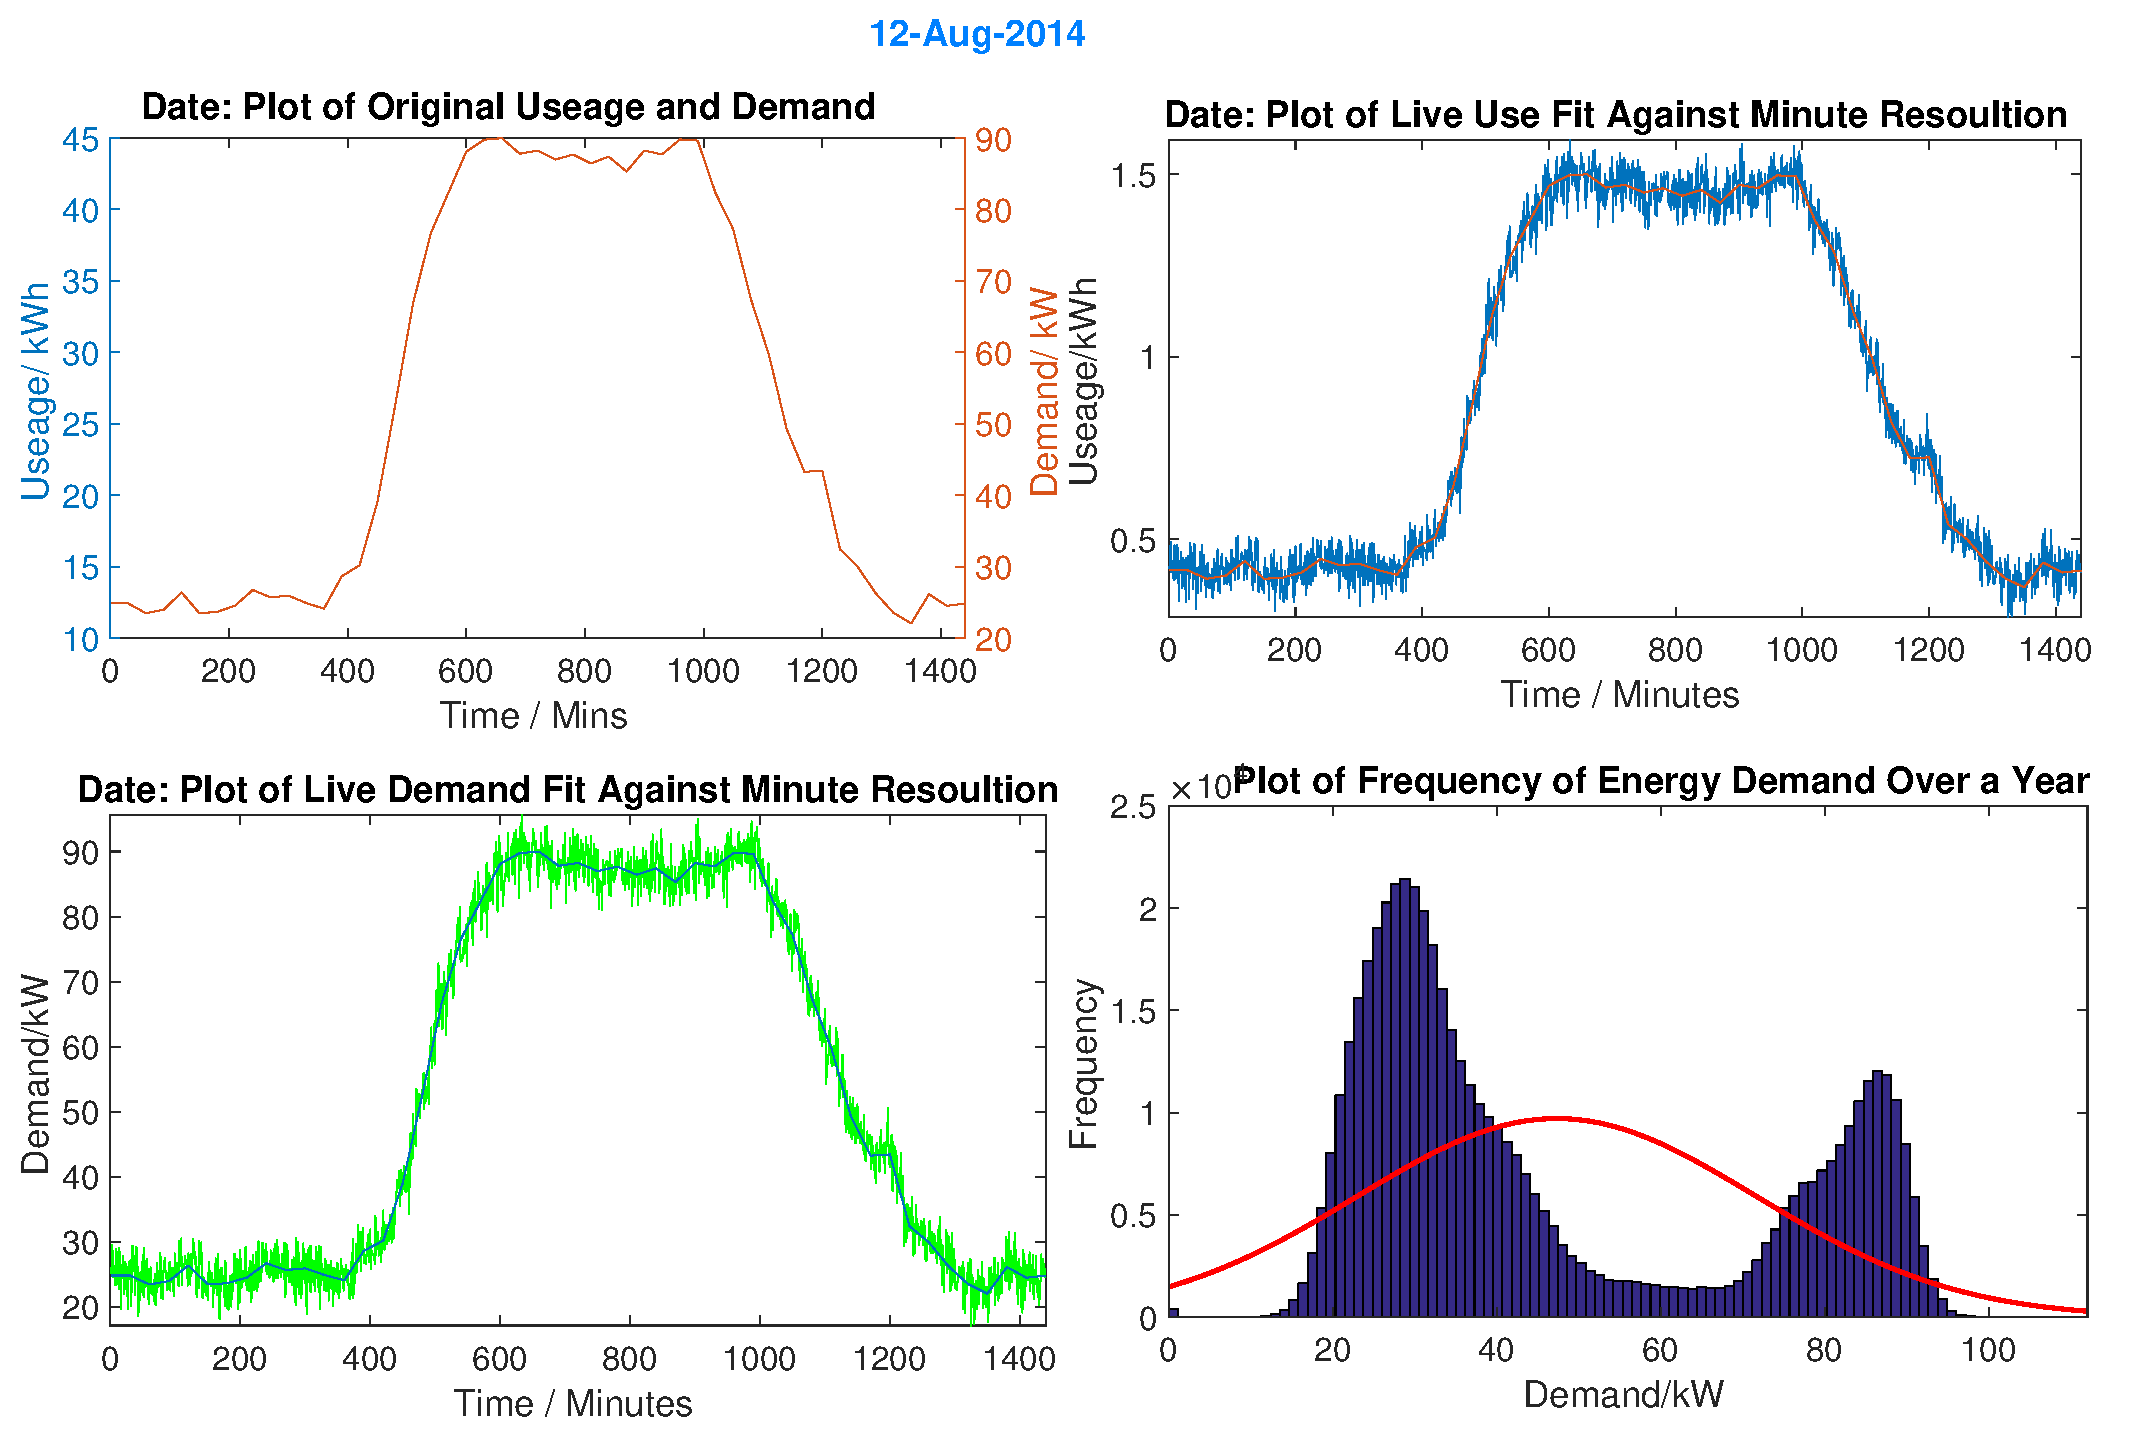
\includegraphics[trim = 0 0 0 0 clip, width=0.8\textwidth]{sendem.eps}
  \vspace{-10pt}
 \caption{Plots of Usage and Demand Profile Generation and Histogram of Year Data}
 \label{sendem}
 \vspace{-25pt}
 \end{figure}

To fully understand the energy profile of the Senate house, histogram
and as a cumulative distribution plots
\footnote{See Figure \ref{loadprofile} in the appendix to see Senate House's load profile}
were used to identify the typical demand of Senate House sees over the
year, as well as the max demand the building experiences
\autocite{combined-heat-power-buildings}. Figure \ref{sendem} shows the
demand profile of Senate House, providing insight into what requirements
a battery system may need. It can be observed from in the histogram,
that the demand of the Senate House typically falls between two points.
One low peak representing morning and evening of 30KW and a second peak
constituting the energy usage in the middle of the day, averaging around
80KW, but rarely ever exceeding 90KW. Insights from the load profile
also identified a battery rated to 40KW would cover, 5000 hours of the
year roughly 55\% of the year's usage.

\subsection{Definition of the New Temple Quarter
Campus}\label{definition-of-the-new-temple-quarter-campus}

Understanding the outline of new campus was required to create a valid
assumption of its energy profile. At the time of writing, no building
plans were available. Instead many assumptions about the likely size and
use of the campus were used to create a representative energy profile
\footnote{See Table ? In the appendix for a breakdown of how the new campus was sized}.

The campus will be designed for \textasciitilde{}1500 resident students,
having \textasciitilde{}5000 staff and students on site during term. A
range of facilities have been proposed for Temple Quarter Campus,
however it is likely that the campus will constitute largely of tutorial
rooms, a few lecture halls and offices. A meeting with John Brenton
\autocite{Jbrentmeet}, made clear that creating an infrastructure to
support postgraduate business studies made the most economical sense,
and is likely to influence the Campus's design.

As tutorial rooms and office are similar to Senate House, It is assumed
that the energy profile of Senate House will be transferrable to the new
campus. It is unlikely the new campus will have any equipment that will
distort the load profile greatly; where the campus is likely to have
improved efficiency through employing the latest technologies in its
construction and services (HVAC). Data on 125 rooms in halls of
residence was also provided, with a higher degree of certainty of its
applicability to the new campus. Footprints of both buildings were
combined with laboratory data, testing the effects labs may have on any
large spikes in energy usage. The final scaling factors used were:

\begin{itemize}
\tightlist
\item
  Senate House (7840sqm) - \textbf{7.9x}
\item
  Hall data (2761sqm) - \textbf{7.6x}
\item
  Lab data (1 Lab Use) - \textbf{4x}
\end{itemize}

\subsubsection{Energy Profile Tool}\label{energy-profile-tool}

Due to energy usage data files beginning on different dates and running
for various periods of time, these records required adjustment to be
correctly scaled and combined. To fully meet the project's outputs and
modelling requirements, a program was created to manipulate various
half-hour energy use files. An algorithm was set up to read the data
dates and then convert this data into realistic demand profile. To
simulate lifetime energy usage, copies of the energy profile were
concatenated for the length of simulation, checking that each year began
on the next day in the week from the end of the previous year. It was
imperative that dates aligned, to make sure results were valid as the
difference in energy usage between weekdays and weekends (see section
\ref{creation-of-senate-house-billing-model}), could cause the total
savings to vary on a seven-year cycle pattern. Figure
\ref{EnergyProfileTool} outlines the logic of this program.

\begin{figure}[H]
 \centering
 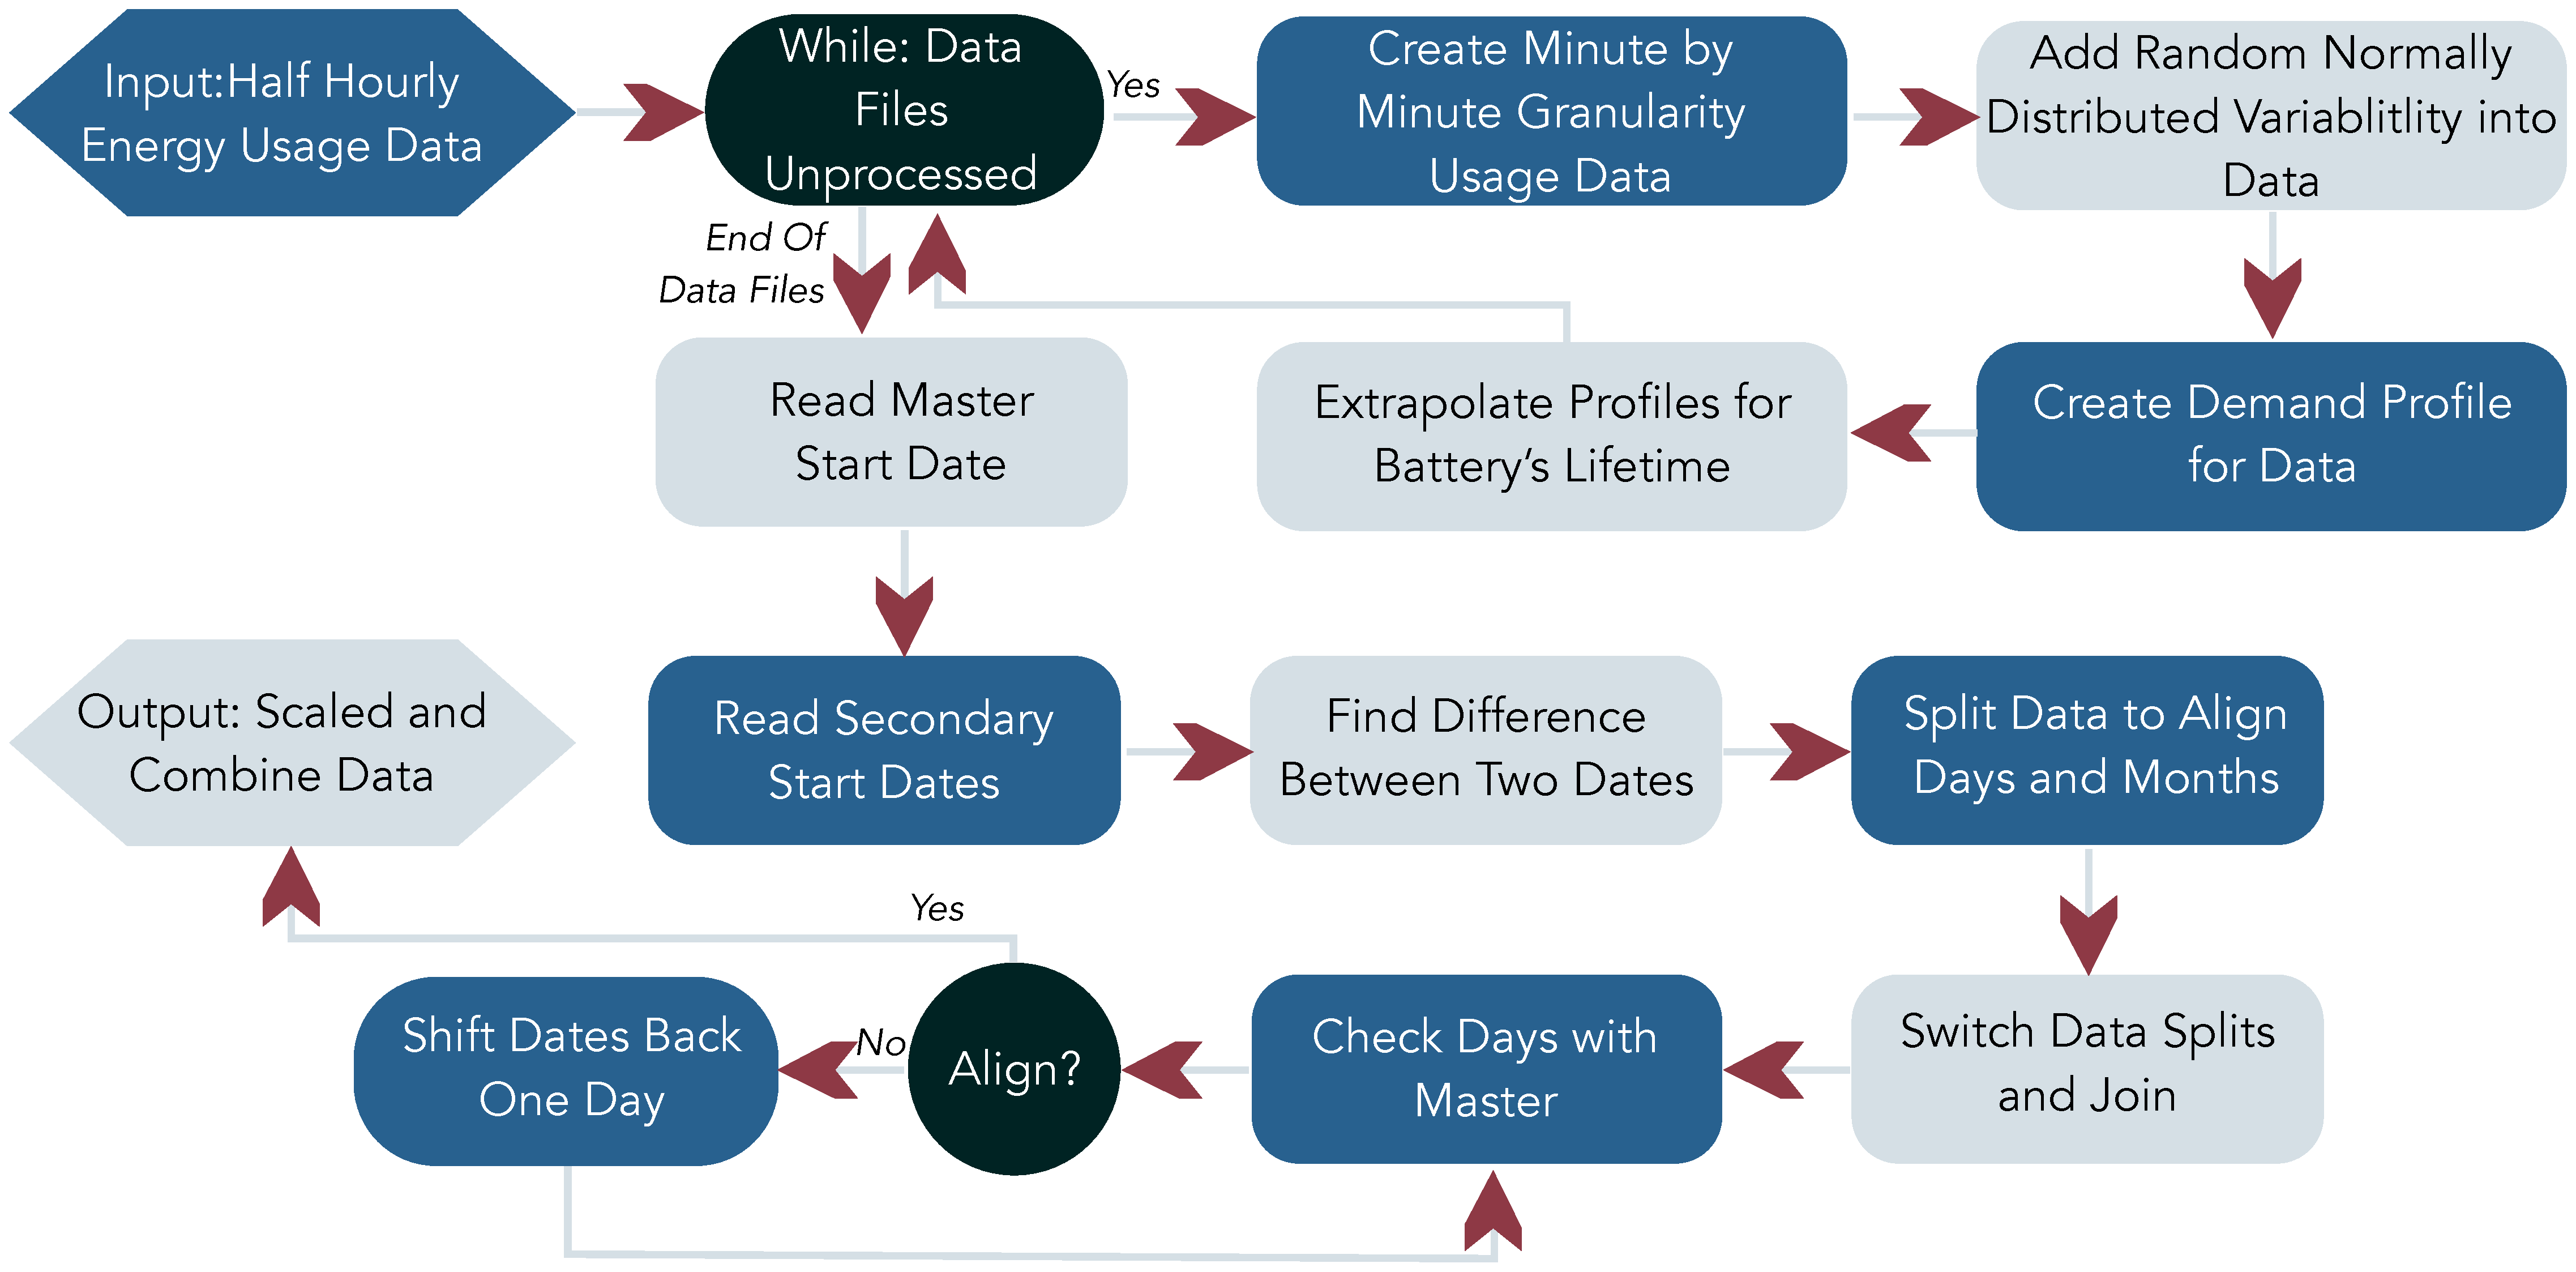
\includegraphics[trim = 0 0 0 0, clip, width=0.85\textwidth]{EnergyProfileTool.eps}
 \caption{Logic of Energy Profile Tool Create New Campus Data}
 \label{EnergyProfileTool}
 \vspace{-20pt}
 \end{figure}

\subsection{Definition of System
Strategies}\label{definition-of-system-strategies}

To fully understand the value of using battery storage, a representative
simulations of how the battery would operate is required. This section
defines the logic define the battery's operation. The model calculates
both economical and technical battery performance based on the chosen
battery strategies. The following section will discuss why the final
strategies were selected, detailing their development.

\subsubsection{Red Rate Charge Avoidance
Strategy}\label{red-rate-charge-avoidance-strategy}

As outlined in section \ref{representative-bill-creation}, using energy
consumed during Red rate periods was considerably more expensive than
Amber and Green periods, making it a prime strategy. By switching the
battery on during Red rate periods, then charging during Green periods,
cost savings of up to 20\% could be made. Currently, for the University,
Red rates apply between 5 and 7 PM on weekdays making it simple to
forecast, alleviating the need for complex prediction systems
highlighted in section
\ref{forecasting-and-the-use-of-ess-in-load-shifting}. During this
period the battery would be drained at a rate up to its maximum output
power; requiring demand and usage data to be checked simultaneously. If
the load exceeded max power, energy supply was capped at this value. The
battery would continue to be drained until either its minimum capacity
was reached, or the Red rate period elapsed. The battery would then be
fully charged during green ensuring all capacity was available for the
next Red rate period is entered. This method was repeated for the
run-length of the simulation.

\subsubsection{Triad Avoidance Strategy}\label{triad-avoidance-strategy}

To correctly understand the effects of TRIAD avoidance in the model,
TRIAD dates needed to be correctly identified. Using \autocite{triad15},
the dates: 4/12/14, 19/01/15, 02/02/15 were used; aligning with the
original Senate House data set as the as a master template for the new
campus (discussed in section \ref{energy-profile-tool}). These dates
were used for the sequential years in the simulation as they were
typical days in which TRIADS would fall. From observation, it was
assumed that there was no increase in the University's usage during
TRIAD periods, allowing for any day within that week to be used. To make
sure these dates did not fall on fall weekends, days were checked and
adjusted accordingly. It is assumed that daily variation in energy usage
is negligible and instead energy trends are seen only on a monthly
basis.

It was observed that TRIAD times all fell into Red rate periods,
corresponding with the Red rate avoidance battery strategy. Using these
dates and the time of 5:30, the TRIAD cost was calculated based on
energy demand (kW). Battery usage was then measured against the TRIAD
cost to understand the reduction in energy demand delivered by the
battery. The reduction in TRIAD rate was a factor of the batteries max
power supply and not capacity; due to the battery would only need to run
for a few minutes to offset this charge.

At the end of each year in the simulation, usage on the three TRIAD
dates were averaged to find the total cost. This was then spread evenly
over the next year in the simulation, representing how TRIAD billing is
split across each monthly energy bill.

\subsubsection{Battery Control Strategy}\label{battery-control-strategy}

The importance of optimising battery longevity was highlighted in
\ref{forecasting-and-the-use-of-ess-in-load-shifting} and
\ref{battery-sizing-and-financial-modelling}. Section
\ref{battery-degradation-parameters}, discussed the different variables
which can affect a battery's longevity. An approximation of the battery
degradation was taken, taking into account the effect of each of these
variables as a battery control strategy.

The rated battery cycle life is taken to be the number of full cycles a
battery can complete before it degrades to 80\% of its original capacity
\footnote{This is quoted to be 5000 cycles for the Tesla Powerpack, see Figure \ref{pp2tab}}.
This figure was used as a measure for how the battery should perform
based on a normal use case. Using this assumption, the battery was
degraded proportionally by the fraction of its current cycle.

\begin{wrapfigure}{r}{0.26\textwidth}
\vspace{-25pt}
  \begin{center}
\includegraphics[trim = 0 0 0 0, clip, width=0.25\textwidth]{BatteryImage.pdf}
  \end{center}
  \caption{Showing Battery Degradation}
   \label{BatteryImage}
   \vspace{-30pt}
\end{wrapfigure}

For each charging iteration, the new max capacity became slightly
smaller, reducing the size of the cycle. A counter was used to sum each
charge, resetting when its value equalled the current cycle size;
signifying one complete cycle. Using this method, battery's were
degraded on their on their use, degrading quicker as they deterioted.
This followed the battery cycle degradation trend shown in figure
\ref{batCapGen}.

By using the cycle-life metric, all battery degradation assumptions were
based on the battery's operation and not the battery's chemistry.
Assumptions on the batteries normal working parameters were made,
limiting the battery to conform to these rules. This would prevent the
battery running in a way that would majorly affect its longevity, making
the prediction more accurate. These restrictions could be made greater
or smaller at the expense of more or less chance of error on the battery
health prediction. The following battery control measured were
implemented:

\begin{itemize}
\item
  \textbf{Reduction in Depth of Discharge}: To reduce wear on the
  battery, the battery was confined to work within 10-90\% of its
  current maximum capacity, allowing a maximum depth of discharge of
  80\%. Draining the battery can cause detrimental effects on the while
  overcharging can also do the same. Working within these two parameters
  follows similar principles applied by Tesla in their electric cars
  \cite{Charging49:online}.
\item
  \textbf{Speed of Depletion}: A battery was never run above its max
  specified power. As the battery was rated at this value, it should be
  designed to cope with this level of use for no longer than 2 hours a
  day. The simulation will analyse the average discharge rate as a
  measure of the validity of the battery health
\item
  \textbf{Temperature}: was assumed to remain within expected bounds,
  based on the assumptions made in section \ref{temperature}. Using the
  Red rate and TRIAD strategies would allow the battery to cool over
  weekends.
\item
  \textbf{Charging}: The battery would only charge during Green periods,
  at a rate which would ensure the battery would be charged fully by the
  next Red period; this was based on the capacity required divided by
  the length of the Green rate period. Section
  \ref{Battery-Degradation-Parameters} suggested that charging at a
  lower speed, particularly during the last 10\% of charge, made a large
  impact on the battery lifetime. It is assumed here that smart charging
  techniques such as trickling (seen on most modern smartphones), would
  be incorporated into the actual battery, but modelling these methods
  would not increase the accuracy of the model, so was been neglected.
\item
  \textbf{Battery Efficiency}: This was regarded in the model by
  multiplying the energy drawn when charging by the additional losses
  caused inefficiencies. This assumption was made as it is likely that
  the battery once charged can supply what it has stored. The Powerpack
  2 integrated inverter, supplies energy in AC, quoting its efficiency
  to this level (see figure \ref{pp2tab}). It is assumed that the quoted
  figure is very representative of the battery's efficiency in the
  system. Efficiency gains could also be achieved by designing the
  system, so it primarily sends power to DC first without transforming,
  this will not be evaluated in this project, see Figure \ref{pp2tab}.
\end{itemize}

\begin{wraptable}{r}{0.42\textwidth}
\vspace{-20pt}
\caption{Tesla Powerpack 2 Specification}
\vspace{-5pt}
  \begin{center}
     \includegraphics[trim = 0 0 0 0, clip, width=0.41\textwidth]{PP2spec.pdf}
  \end{center}
  \vspace{-20pt}
  \label{pp2tab}
\end{wraptable}

The model was run until the either runtime elapsed or the battery
reached its end of life value (80\%), allowing results to be comparable.
There are examples of batteries being used beyond their end of life
cycle. Renault and connected energy have been investigating using the
end of life Li-ion car batteries in home use applications
\cite{Renaultt62:online}, \cite{UsedRena38:online}. It is believed there
is still plenty of life remaining, and the increased probability of
failure is less of a problem when used for bill reduction purposes. In
the case of the new campus, there are little-associated costs with
batteries after they have been installed if the battery has paid itself
back, the battery will continue to generate profit. If unpredictability
is seen to be an issue, this may be the case if emergency power is seen
as a key value of having the battery, then it may be possible Analysing
this value is out of scope for this project so an end of life battery
was be classed as having no value.

\subsection{~Input Parameters and Multi-Battery
Simulation}\label{input-parameters-and-multi-battery-simulation}

To understand the optimum battery type for a given scenario, and then
infer the total savings that the battery could generate; a large array
of different batteries with different power ratings and capacities were
modelled. Using actual data from Tesla \cite{Powerpac23:online}, the
real costs of the different battery specifications were modelled. To
find trends in the different battery types, the modelled required
iterating through numerous different battery specifications. To reduce
computation time, parallel computing was implemented to iterate each
discrete battery scenario in the 0D model.

The following diagram depicts the model of the entire multi-battery
system.

\begin{figure}[H]
 \centering
 \includegraphics[trim = 0 0 0 0, clip, width=0.8\textwidth]{largelogic.eps}
 \caption{Logic Diagram For Multi-battery Simulation}
 \label{largelogic}
 \end{figure}

To comply with the requirements set in section
\ref{model-development-requirements} The following methods were used to
optimise the performance of MATLAB model.

\begin{itemize}
\tightlist
\item
  \emph{Vectorisation}: storing data within multidimensional arrays and
  using vector operations
\item
  \emph{Variable Initialisation}: all matrices were initialised to
  reduce memory.
\item
  \emph{MATLAB Function Reduction}: functions such as linear
  interpolation are cumbersome. These were recreated and simplified,
  solving tasks more efficiently.
\item
  \emph{Parallel Processing}: Multiple cores on the processor were used
  to iterate through independent battery specifications in large
  multi-battery simulations. To achieve this successfully, code was
  rewritten to make all events discrete, substituted methods such as
  \texttt{while} and \texttt{break}. For large multi-parameter
  simulations, this can increased the processing time significantly,.
\item
  \emph{Profiler Tool }: Within MATLAB, the performance of code can be
  measured in the amount of time it takes to run. This tool was used to
  identify bottlenecks within the model.
\item
  \emph{Single Integers}: Single integers are half the size of double
  integers, the default storage method for data within MATLAB.
  Double-precision floating point numbers allow the CPU to handle very
  large values. As this level of accuracy is unnecessary, use of 32bit
  single integers increased performance \autocite{getreuer5685writing}.
\item
  \emph{Do Not Repeat Yourself (DRY)}: Coding technique to improve
  readability and performance of code, through use of functions.
\end{itemize}

The result of this method reduced processing time per battery from
\textasciitilde{}110 seconds to under 10 seconds. This was crucial in
allowing the 113 different battery simulation run quickly. The runtime
of the multi-scenario program was reduced to 220 seconds. This allowed
different sensitivities studies to be run, greatly improving the
functionality of the tool.

\section{Validation of Model}\label{validation-of-model}

\subsection{Data File}\label{data-file}

By using the model with real data first taken from Senate house, the
tool which creates live data could be validated through integration and
direct comparison to the original usage data. As no data could be
gathered on how the demand profile looks for Senate house, assumptions
were made on the type of operations the building fulfils (see the table
below); this was compared to demand data at Princeton
\autocite{LiveData90:online}. Section \ref{battery-model-definition}
describes how the model was initially tested on Senate House to validate
whether the model produced expected results. After being validated on
Senate House the model was then run of the new campus energy profile.

\subsection{Assumptions and
Limitations}\label{assumptions-and-limitations}

Table \ref{BatterAssump}, summarises all the assumptions discussed in
section \ref{battery-model-definition}. To create a valid model, all
assumptions must be based on logical expectations on all parameters that
may effect the system, thereby using the following assumptions, the
model is validated.

\begin{table}[H]
\vspace{-10pt}
\caption{Showing All Assumptions Made for Simulation}
\vspace{-5pt}
 \centering
 \includegraphics[trim = 0 0 0 0, clip, width=0.95\textwidth]{assumpp1.pdf}
 \label{BatterAssump}
 \vspace{-30pt}
 \end{table}

\begin{table}[H]
 \vspace{0pt}
  \centering
  \includegraphics[trim = 0 0 0 0, clip, width=0.95\textwidth]{assumpp2.pdf}
  \vspace{-20pt}
  \end{table}

The model is limited to working to these parameters only. Section
\ref{ease-of-development}, set an objective for the model to be
developed so these parameters can be easily changed, allowing for the
model to be easily customised to work with a different set of
assumptions. Peaks in demand being higher than modelled, energy pricing
changing and DOD and discharge rate effect on capacity all have high
levels of uncertainty in the model. These were sensitivity checked to
understand the effects of these assumptions being incorrect.

\section{Results}\label{results}

The objective of this report was to evaluate whether there is the strong
business case for investing in energy storage technology for the New
University Campus. This section analyses the data gathered from the
zero-dimensional model, discussing the value which optimum batteries
specifications could bring to the new Temple Quarter campus. Figures
\ref{histredload} and \ref{redloadperc}, describes the energy profile
for the new campus's usage during Red rate periods.

\begin{figure}[H]
\centering
\begin{minipage}{.495\textwidth}
  \centering
 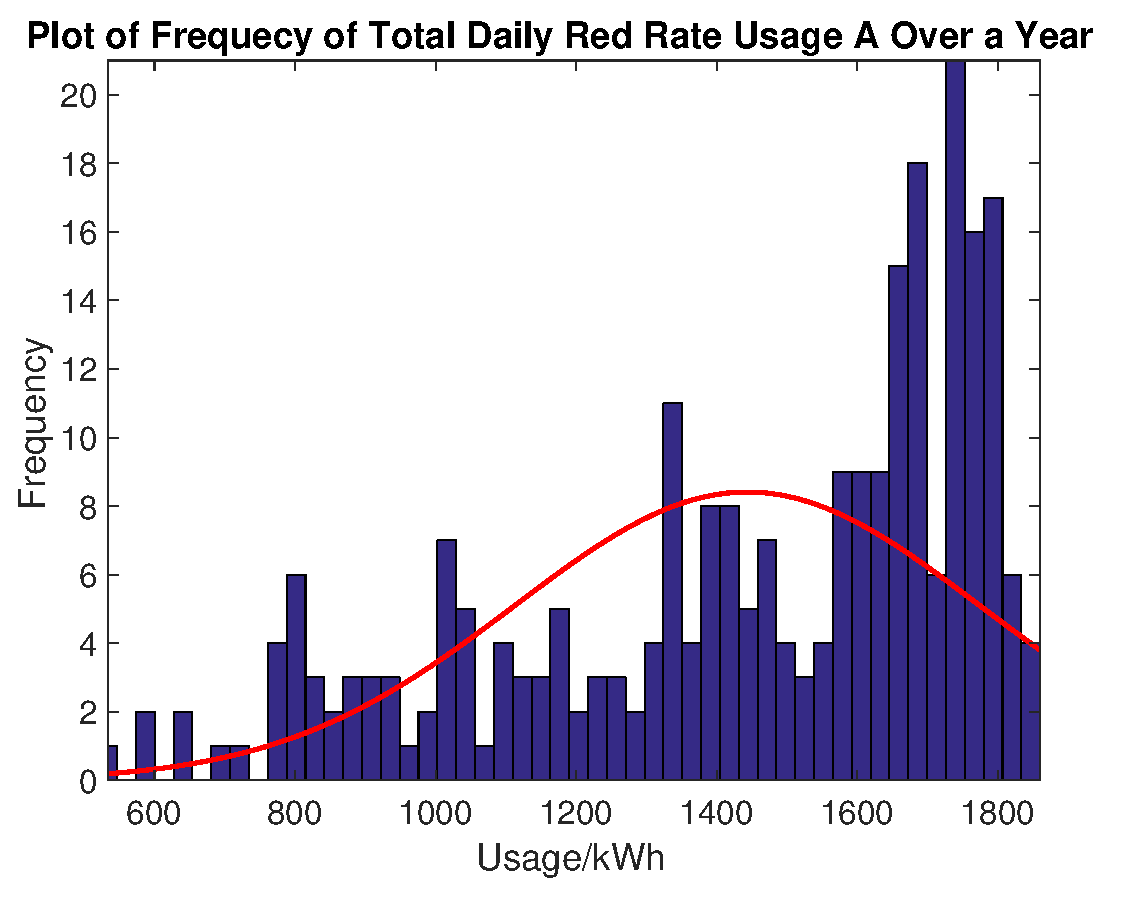
\includegraphics[trim = 0 0 0 0, clip, width=1\textwidth]{histredload.eps}
 \vspace{-20pt}
 \caption{Histogram Showing Red Periods Total Daily Usage Frequency}
 \label{histredload}
\end{minipage}
\hfill
\begin{minipage}{.495\textwidth}
  \centering
 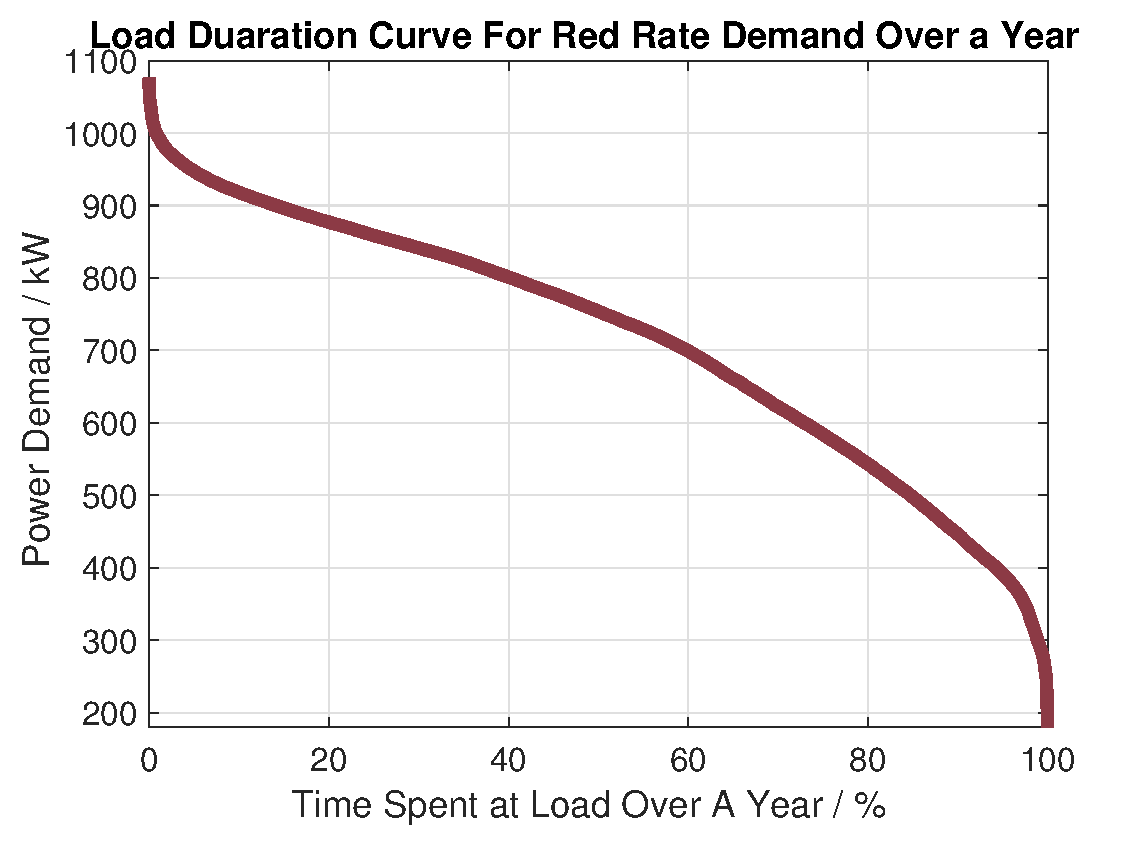
\includegraphics[trim = 0 0 0 0, clip, width=1\textwidth]{redloadperc.eps}
 \vspace{-20pt}
   \caption{Time Spent at Power Demand Level}
  \label{redloadperc}
\end{minipage}
\vspace{-30pt}
\end{figure}

These energy profile plots, described the range of battery
specifications which should be simulated. Figure \ref{histredload}, that
how a battery with a usable capacity greater than
\textasciitilde{}1800kWh will have excess capacity to demand. By taking
into account end of life degradation, battery's up to and end of life
capacity of 2000kWh were modelled. Figure \ref{redloadperc}, describes
the percentage of time the battery would spend at max load. A battery
rated at 920kW would be only run at max load 10\% of the time. As
discharge rate effects capacity, battery's rated up to 1300kW were
simulated. Based on this analysis 65 different Powerpack 2 battery
specifications were identified as plausible solutions.

A 25 year runtime period was used to evaluate the battery performance
over \footcite[See Page 27 of][]{heatcibse}; chosen on the assumption
that most technology in the building will be replaced by this point, as
the building begins to receive some refurbishment. Li-ion battery
technology will have also significantly advanced, or at least drop
significantly in price
\footnote{See Figure \ref{mckBatPrice} for a prediction in battery prices}.
Using a set period will also reduce uncertainty in battery health and
prevent favouritism for larger batteries. An investor is unlikely to
look beyond 25 years, so savings made after these periods will not be
considered. The following results will talk through the three key value
measurements discussed in section \ref{battery-economics}.

\subsection{Total Savings and Payback
Period}\label{total-savings-and-payback-period}

Figure \ref{SRTS2} shows the parabolic shape with a local maximum
between the battery size and the total savings. For the new campus, a
battery size of around \textasciitilde{}2.2MWh generated the maximum
total savings over the simulation run time. In contrast, Figure
\ref{SRPB2}, highlights that a much larger range of batteries fell close
shortest payback time of 6.3years, where power and capacity increased
proportionally.

\begin{figure}[H]
\centering
\begin{minipage}{.495\textwidth}
  \centering
   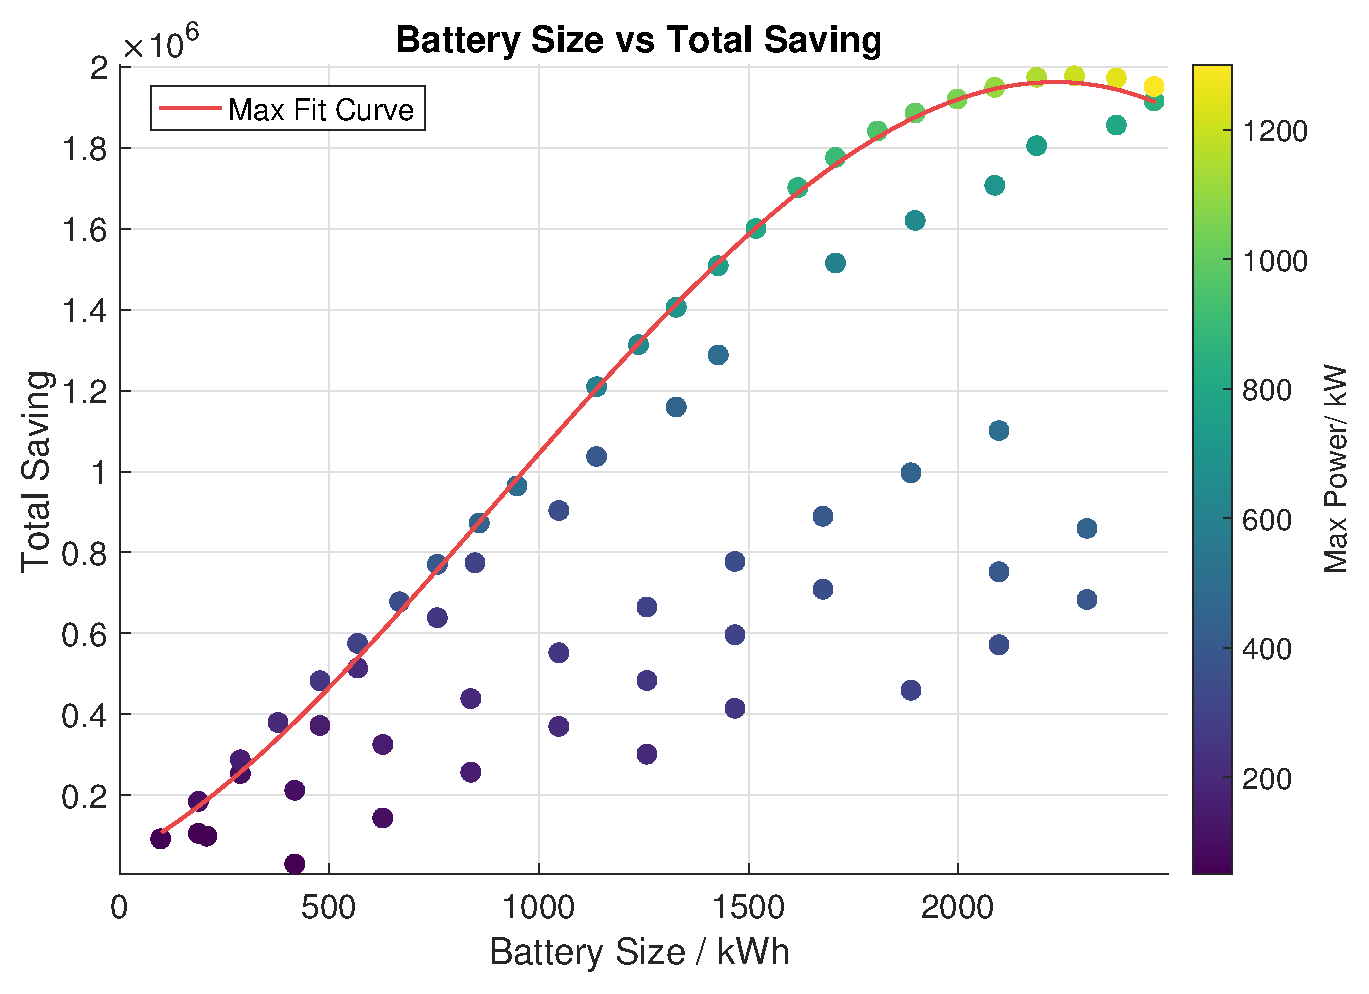
\includegraphics[trim = 0 0 0 0, clip, width=1\textwidth]{batsts.eps}
 \caption{Battery Size Vs Total Savings}
 \label{SRTS2}
\end{minipage}
\hfill
\begin{minipage}{.495\textwidth}
  \centering
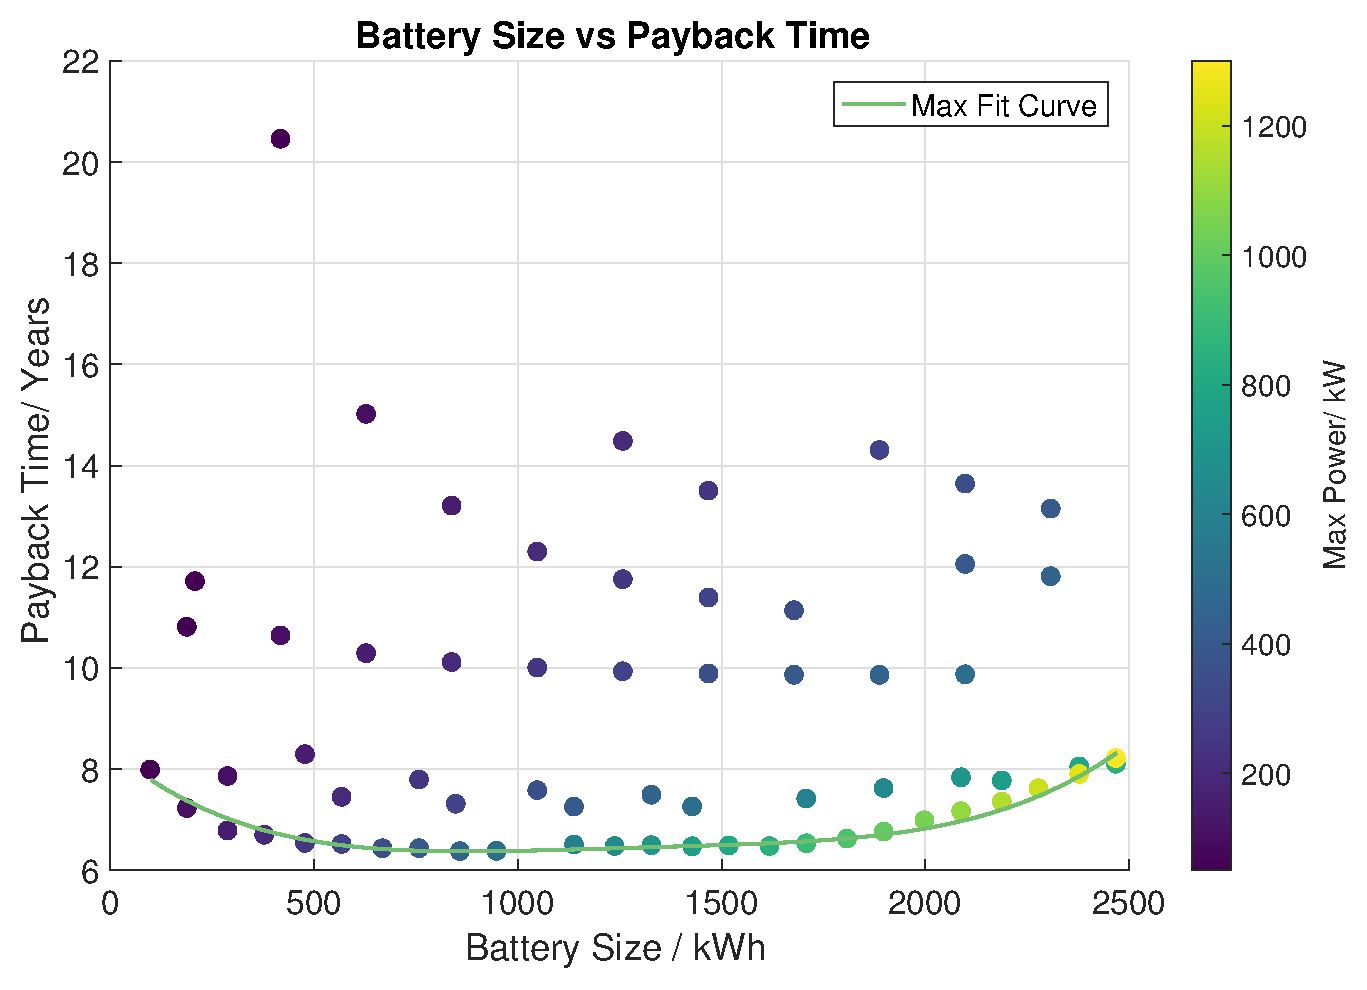
\includegraphics[trim = 0 0 0 0, clip, width=1\textwidth]{batspb.eps}
   \caption{Graph of Battery Size vs PayBack Time}
  \label{SRPB2}
\end{minipage}
\vspace{-10pt}
\end{figure}

Figures \ref{SRTS2} and \ref{SRPB2}, begin to give a good insight into
the financial performance of the battery, however, presented in this
form, it difficult for a designer to choose the optimum battery. To make
the results more useful, an algorithm was made, which generated best-fit
plots over the maximum battery specifications for the different total
saving and payback time plots. Figures \ref{SPA2} shows how these curves
plotted over the maximum values.

\begin{figure}[H]
\centering
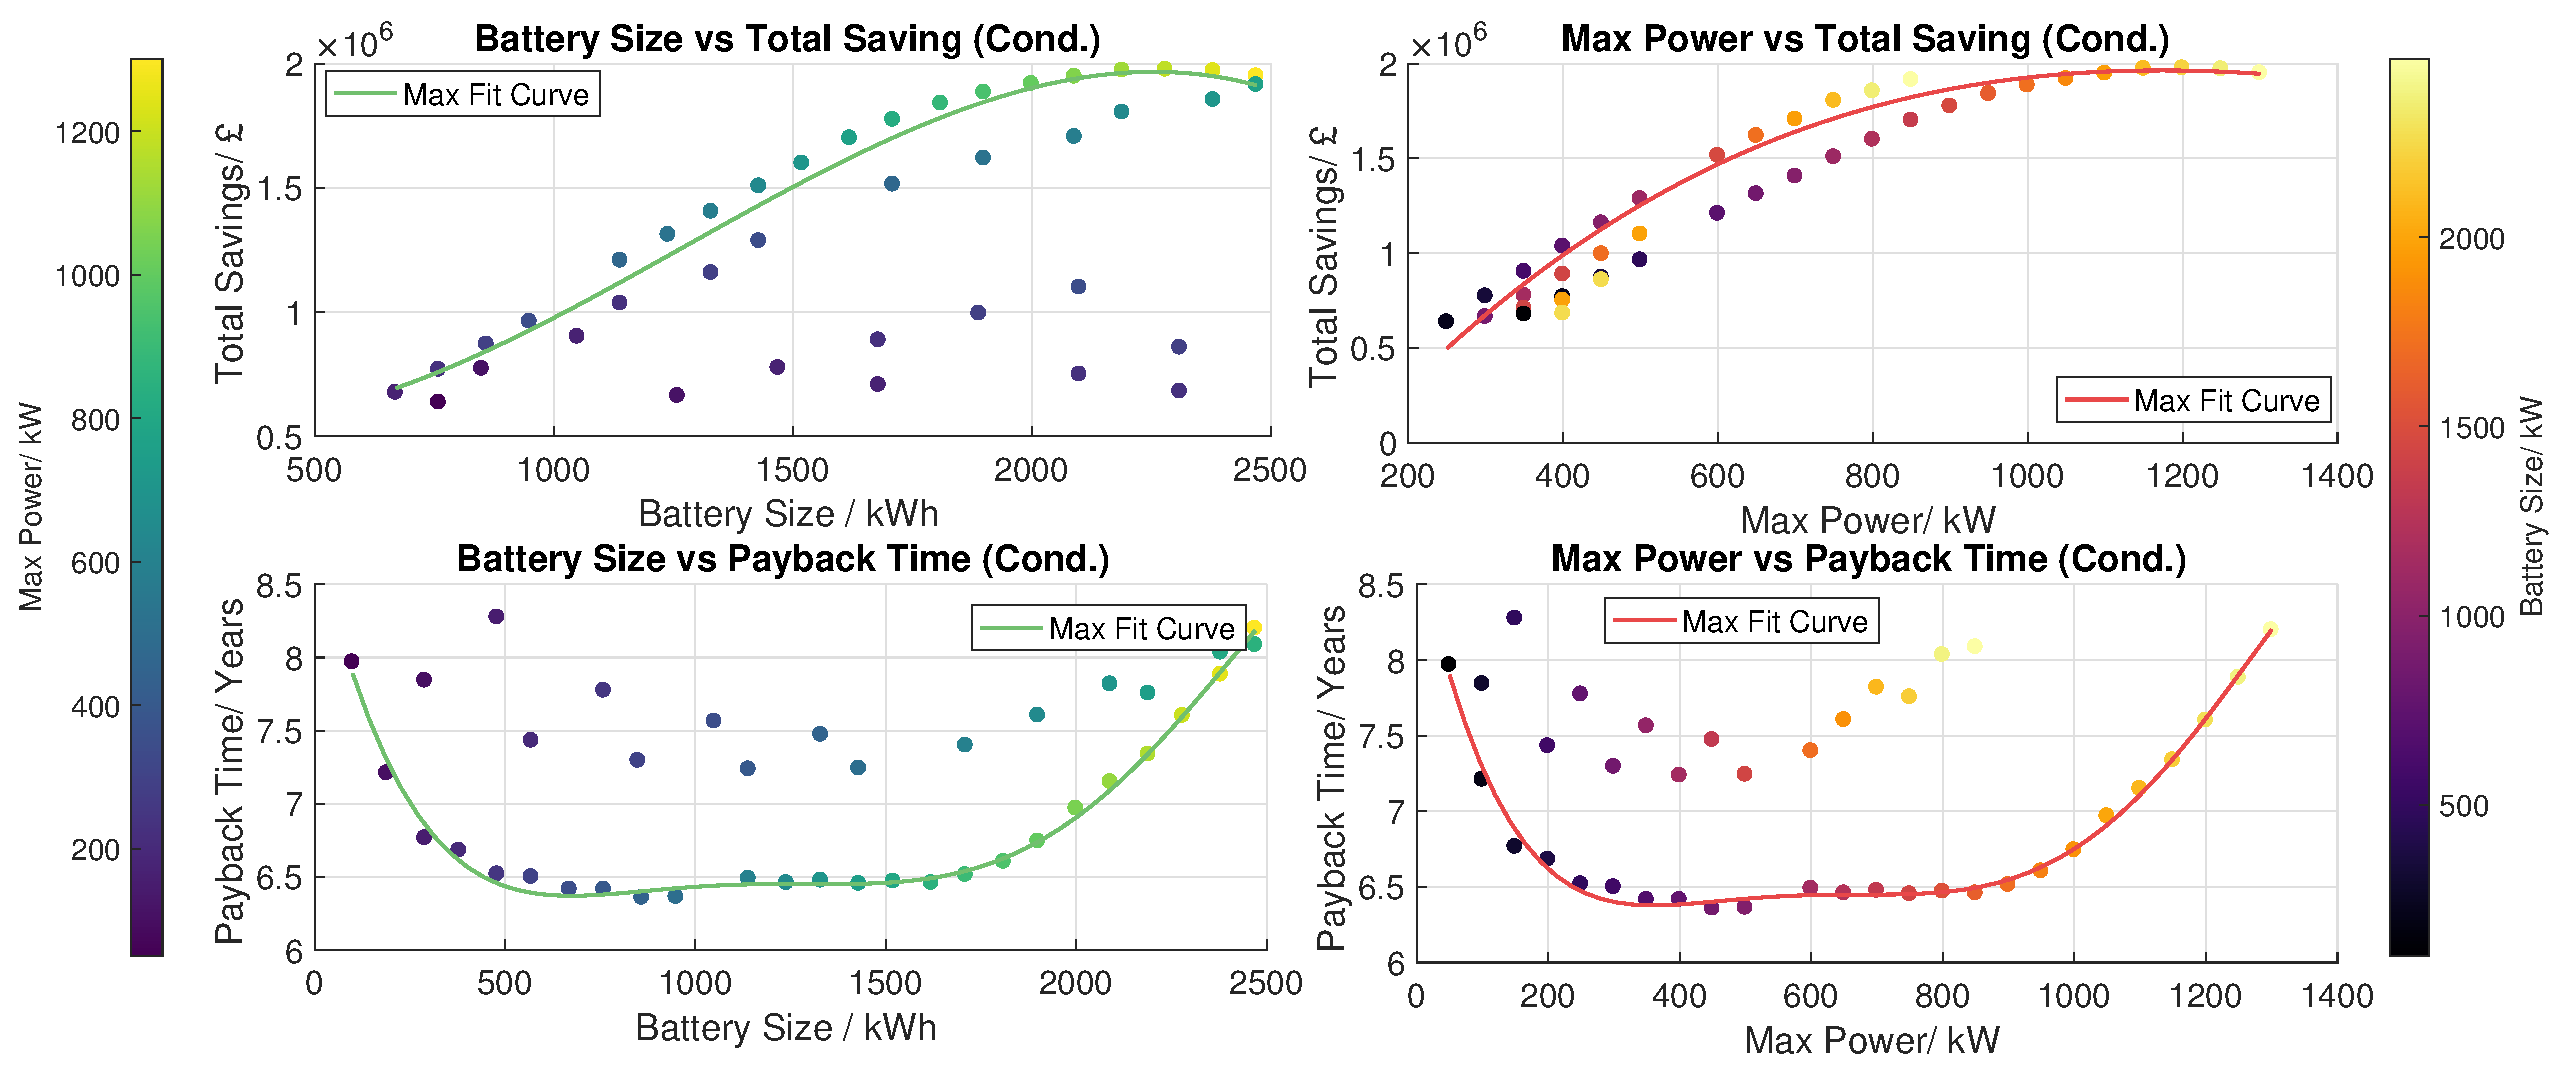
\includegraphics[trim = 0 0 0 0, clip, width=1\textwidth]{mxfit.eps}
\caption{Graph Showing Top 40 Batteries with Fitted Curves for both Payback Time and Total Savings}
\label{SPA2}
\vspace{-20pt}
\end{figure}

By superimposing these max-fit curves, a graphical tool was created,
allowing a designer to visualise the tradeoff between total savings and
payback time, shown in Figure \ref{SRTSPB5}. A small region around the
cross over point of the two plots shows the specifications of the
optimum batteries. By creating a set of rules (e.g.~the battery must
have a payback period less than seven years), all the solutions become
immediately apparent. A small shortlist of the batteries can be made,
referring back to the original list of Powerpack specifications.

\begin{figure}[H]
 \centering
 \includegraphics[trim = 0 0 0 0, clip, width=1\textwidth]{mxfitplt.eps}
 \caption{Comparison Between Fit Curves for Payback Period and Total Savings}
 \label{SRTSPB5}
 \vspace{-20pt}
 \end{figure}

Analysing Figure \ref{SRTSPB5}, the regions where the best trade-off
between payback time and total savings (around where the two plots
intersect) has been highlighted. The results show that a battery around
1762kWh and 744.4kW, produces a good compromise. Increasing capacity
beyond increases total saving at the result of quickly decreasing the
pay back period. Alternatively, when looking at max power, payback time
is increases slightly for as power decreases. Up top 950kW, total
savings dramatically increase, with very little decrease in payback
time. The green region highlights the region after the intersection
point, showing a battery larger than 745kW but less that 950kW, is
optimum.

Measuring the payback period is necessary when evaluating the risk of
investing in a battery. The longer the payback time, the greater the
risk in either the battery failing or regulation changing diminishing
the batteries value
\footnote{See Table \ref{AdChalltab} for a more detailed description of the challenges that an ESS system faces}.
The Powerpack 2 specifications modelled, have a 10 year warranty; this
eliminates any risk if the battery were to fail before this period.
Changes in energy billing are therefore the biggest risk the technology
faces. Energy contracts typically last no longer than four years
\cite{wpMWMD}, after which a change in pricing scheme could reduce the
battery's value to zero. Knowing that \(\frac{2}{3}\) of the investment
has a very low risk of uncertainty rather than \(\frac{1}{2}\), makes
the investment much more attractive. These factors should be considered
when choosing the design region of battery selection. For a structural
investment, a payback period between 5 and 7 years is deemed good. The
optimum battery payback time is 6.3 years falling within this range.
From this analysis investing in Li-ion appear feasible.

\subsection{NPV}\label{npv}

Net present value was the second method used to assess the battery
systems value. As long payback periods are inherently risky, NPV uses
discount rates to devalue cash that is made further in the future. As
discussed in section \ref{net-present-value}, the Internal Return Rate
was found. This calculation found for the range of battery assessed that
the average IRR was 11\%,falling between 2 and 15\%. Three discount
rates of 3\%, 7\% and 12\% were selected to understand the value of the
different batteries based of the IRR calculation. Figure \ref{SRNPV1}
shows the net present values of the various simulated batteries at these
different rates.

\begin{figure}[H]
 \centering
 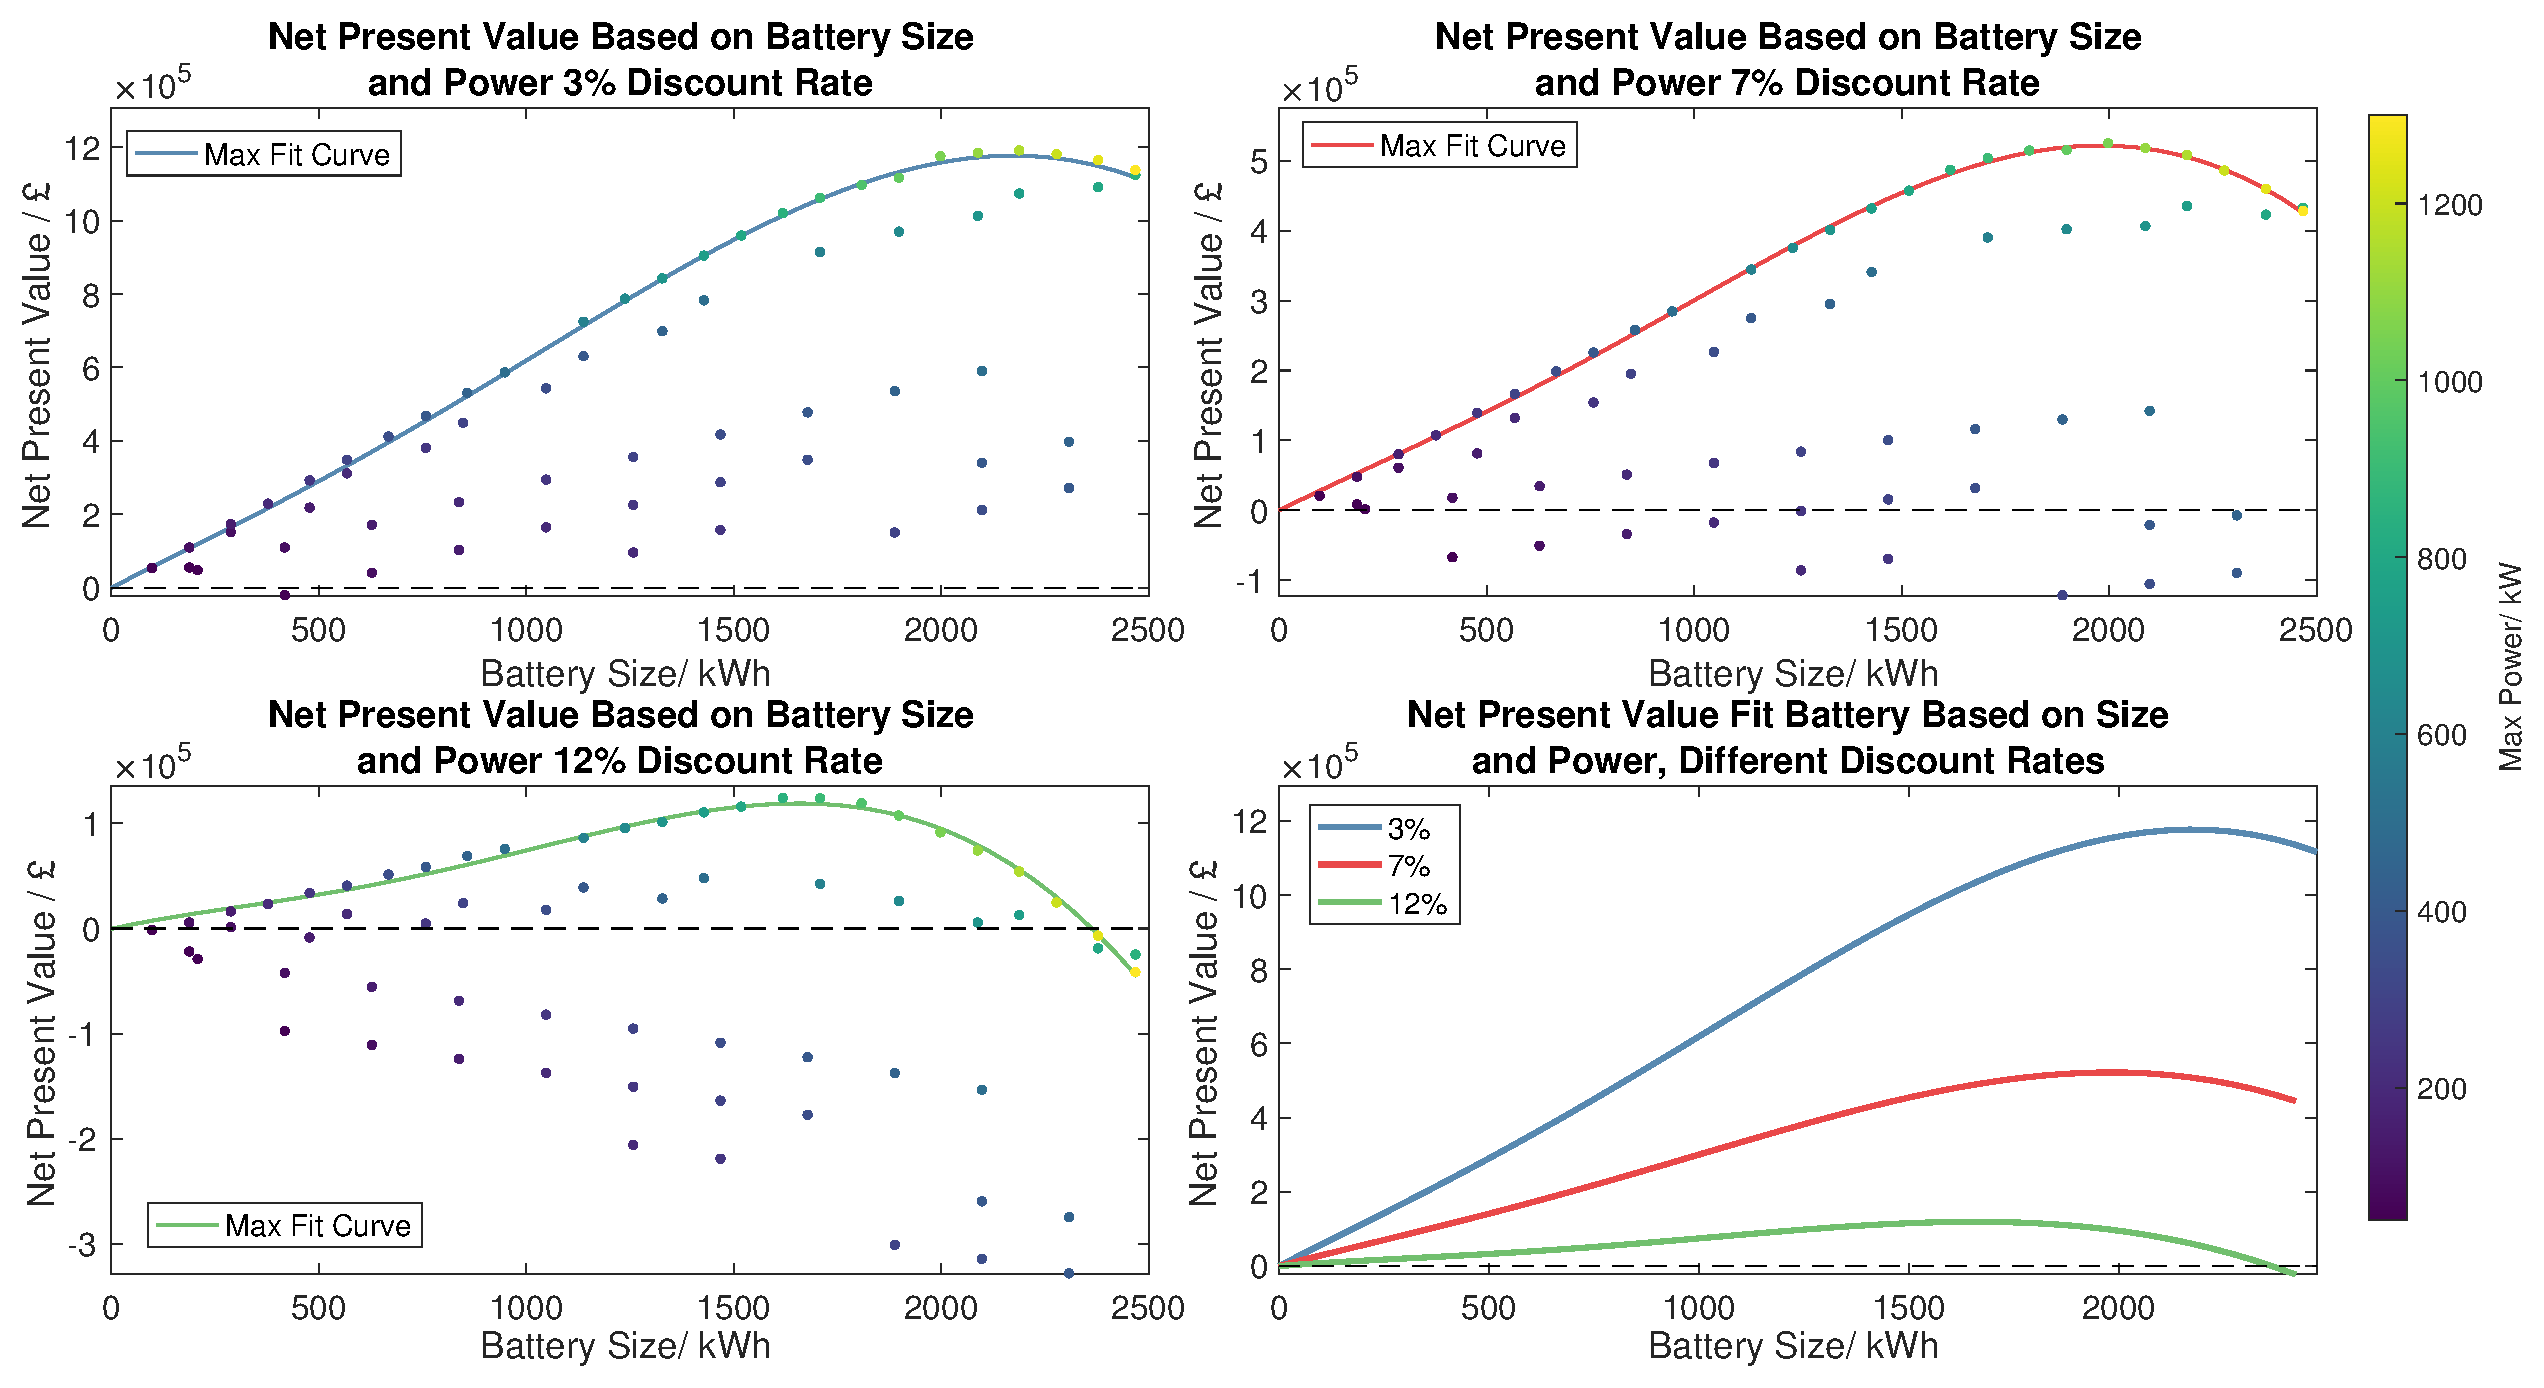
\includegraphics[trim = 0 0 0 0, clip, width=1\textwidth]{npv1.eps}
 \caption{Net Present value at Different Discount Rates - Comparison}
 \label{SRNPV1}
 \vspace{-20pt}
\end{figure}

Using the different NPV rates, presented conflicting optimum batteries.
Increasing discount rate favoured smaller. Looking across the result of
it was decided that a batteries a 7\% discount rate the following
assumptions:

\begin{itemize}
\tightlist
\item
  \textbf{Battery Health}: As the battery will degrade each year until
  it reaches its end of life value, an assumption can be made that the
  value of the asset decreases proportionally to the battery's health.
  Looking at the optimum battery at a discount rate of 7\% (see Table
  \ref{BestNPVTable} below), it can be seen that the specific battery
  ran for 4904 cycles. Based on this assumption the value of the battery
  would be 98\% of its original value, equating to a discount rate of
  \textasciitilde{}3.92\% over the 25 year period. As each battery
  degrades differently, the discount rate due to battery healthy can be
  approximated to 4\%.
\item
  \textbf{Inflation}: Inflation is another factor of the discount rate.
  For the UK, this rate has varied between -0.1\% and 3.5\% for the last
  five years \cite{UnitedKi95:online}. It is expected that the price of
  energy bills will increase with inflation, therefore this interest was
  neglected.
\item
  \textbf{Interest Rates}: Discount rates can be used to incorporate
  interests on loans. As the battery would be purchased at the same time
  as the rest of the new campus it is assumed that the battery will be
  bought under the new campus's mortgage; keeping the interest rate low,
  approximated to 3\%.
\end{itemize}

Using these approximations gives a discount rate of around 7\% shown in
figure \ref{SRNPV1}.

\subsection{Battery Health Analysis}\label{battery-health-analysis}

In order to reduce computational time and simplify the model,
assumptions were made to confine the battery to never work outside of
normal working parameters. Section
\ref{battery-lifetime-assessment---understanding-battery-degradation},
discussed how discharge time and depth of discharge effect the battery
lifetime. Based of experimental data, equations for how these factors
effect were found. The way the model was created to measure average
depth of discharge and discharge time, allowing the effect of these
parameters to be analysed after completing the simulation. Understanding
the effect of these parameters increases the validity of results. Figure
\ref{DOD2mbs} and \ref{Dist1} show the trend between depth of discharge
and discharge for the different batteries.

\begin{figure}[H]
\centering
\begin{minipage}{.495\textwidth}
  \centering
  \includegraphics[trim = 0 0 0 0, clip, width=1\textwidth]{DOD1bs.pdf}
 \caption{Depth of Discharge For Battery Lifetime}
 \label{DOD2mbs}
\end{minipage}
\hfill
\begin{minipage}{.495\textwidth}
  \centering
   \includegraphics[trim = 0 0 0 0, clip, width=1\textwidth]{Dist1bs.pdf}
   \caption{Expected Capacity Offset Due to Discharge Rate and Depth of Discharge}
  \label{Dist1}
\end{minipage}
\vspace{-10pt}
\end{figure}

The patterns observed in Figures \ref{DOD2mbs} and \ref{Dist1} occur due
to the difference between maximum power and maximum capacity. Comparing
this result to Figure \ref{SRTS2}, it can be seen that the batteries
achieving the maximum total savings have DOD greater than 70\%, but are
not always fully discharged. Batteries appear to fall into two
categories; one of high mean depth of discharge between 70-80\% and one
with a mean depth of discharge around 50\%. This is a result of the
relationship between capacity and max power, limiting the possible depth
of discharge that the battery could reach in the two hour red rate
period. With regards to the discharge rate in Figure \ref{Dist1}, As
capacity increases, discharge rate tends also increase, almost doubling
against the high power lower capacity batteries.

Using the polynomial equations outlined in Figures \ref{disRate},
\ref{SoCgraph} and an additional performance parameter describing a more
realistic end cycle life size was found based on these two measurements.
The results are shown in Figure \ref{capnew}.

\begin{figure}[H]
 \centering
 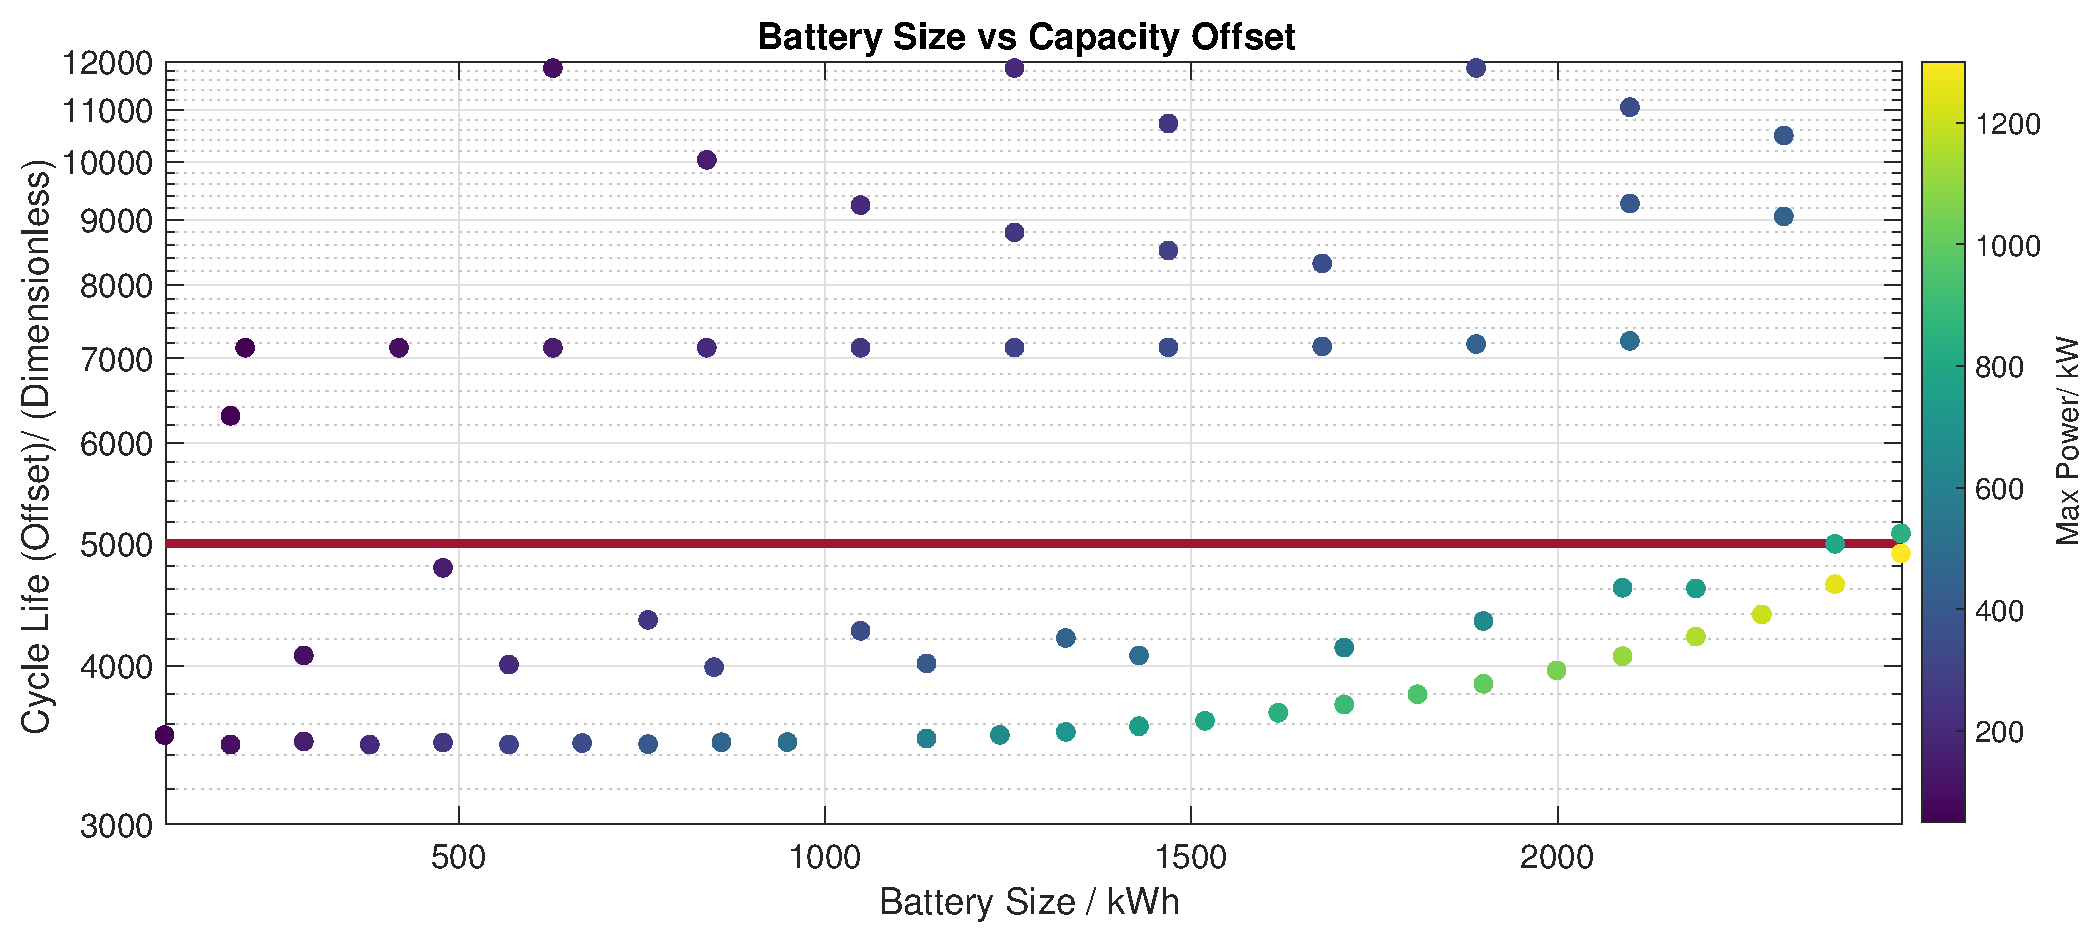
\includegraphics[trim = 0 0 0 0, clip, width=1\textwidth]{capnew2.eps}
 \caption{Showing the Expected Effect of Depth of Discharge and Discharge Time on Predicted Cycle Life}
 \label{capnew}
 \vspace{-20pt}
 \end{figure}

It is clear from Figure \ref{capnew} that taking into account DOD and
discharge time , the lifetime of the battery can either be reduced or
increased significantly. As not all batteries will fully degrade by the
end of the 25 year lifetime, slightly reduced capacity may not be a
problem as the battery should still be functional beyond the end of life
value. From research, it appears depth of discharge can have a more
dramatic effect on the batteries lifetime. To make experimental effects
of DOD comparable for the Powerpack, a conservative assumption of the
battery being rated at 70\% DOD was used. \cite{Teslawil27:online},
however notes that it is possible higher DOD were used to achieve the
5000 cycle life. This would decrease the effect of DOD significantly,
meaning many more batteries would increase in cycle life rather than
decrease. For both these reasons it is unclear whether error in
predicting battery will have a significant effect on the battery's
value.

\subsection{Discussion on Optimum
Battery}\label{discussion-on-optimum-battery}

Table \ref{Bestbat}, show the optimum battery configurations based on
the metrics discussed perviously.

\begin{table}[H]
\centering
\caption{Table Showing the Best Battery Results Comparing the different Economic Measurements}
\includegraphics[trim = 0 0 0 0, clip, width=0.8\textwidth]{topbatstab.pdf}
\label{Bestbat}
\vspace{-20pt}
\end{table}

The following observations can be made on the results:

\begin{itemize}
\tightlist
\item
  The difference in NPV between the best NPV, total savings and max plot
  values is around £40,000, this is relatively marginal against the
  total cost of the investment
\item
  A difference of only a years payback time can be observed by all the
  best performing batteries.
\item
  All the batteries are run towards their maximum working threshold with
  high DOD and mean discharge times
\item
  The maximum plot specification battery gives the highest Return on
  Investment (ROI), this measure helps understand how much money is
  made, compared to how much was invested.
\item
  Annualised savings of all the battery excluding lowest payback ranges
  by £6,000 only. Between max plot and total savings, an increase in
  35\% in upfront cost creates only 9\% more yield a year.
\item
  Selecting a battery based on the lowest payback period has a
  significantly lower NPV and the likelihood of it failing before it
  reaches 5000 cycles is likely
\item
  By selecting the battery with the largest total savings has the
  highest probability of not wearing out before it reaches the end of
  life
\end{itemize}

\subsection{Sensitivity on Key
Assumptions}\label{sensitivity-on-key-assumptions}

\begin{itemize}
\tightlist
\item
  Graph of effect of peak demand rise by 25\%
\item
  Graph on the effect of change in pricing structure - decrease DUOS -
  increase Capacity ?
\end{itemize}

\section{Conclusions and Future Work}\label{conclusions-and-future-work}

\subsection{Conclusions on Modelling
Tool}\label{conclusions-on-modelling-tool}

\begin{itemize}
\tightlist
\item
  This project set out to create multiple tools that would be useful in
  both evaluating the value of a battery system whilst being flexible
  tools that can be used in the 5th year group project.
\item
  \emph{Energy Profile Tool:} to build and understand the New University
  Campus's Demand
\item
  \emph{Optimised Battery System Model:} producing best storage
  solutions based on energy profile tool
\item
  \emph{Business case:} for battery technology investment
\end{itemize}

\subsection{Conclusions on Results}\label{conclusions-on-results}

\begin{itemize}
\tightlist
\item
  Model confirms that it is financially feasible to purchase and use a
  battery to reduce energy bills
\item
  Optimum battery can be selected using different values metrics based
  on the usage profile inputed.
\item
  A 7 year payback period is lower than warranty on the battery,
  eliminating any risks in incorrectly modelling the batteries
  degradation
\item
  After the battery has paid itself back there is nothing stopping it
  continuing to run until it ceases to function. Little maintenance is
  required after its is installed, so nearly all savings are instantly
  realised, this means the battery could theoretically continue to
  generate savings for the lifetime of the building (50 years)
\item
  Due to the modular design of the Tesla Powerpack, after the system is
  initially installed it is feasible to swap the batteries out after
  they have worn out.
\item
  The simulation is ran for a long period of time (25 years), there is a
  large amount of unpredictability particular in energy tariffs, that
  could dramatically alter the value of the battery system over it's
  life time. \hl{the sensitivity study showed.....}.
\end{itemize}

\hl{Refer Back To Challenges and Compare how these challenges are either overcome or still barriers}

\begin{itemize}
\tightlist
\item
  \emph{Costs of Purchase too high}: the model proves that this barrier
  has been over come. As the battery will be purchased as an asset along
  with the buildings, land and other equipment that will be purchased
  for the new campus, it can be assumed that a very low interest rate
  will be taken on the battery.
\item
  \emph{Lifetime/ longevity of the battery too low}: Model of
  degradation shows that the lifetime of Li-ion is now feasible based on
  the battery being run in a controlled manner optimising it's
  longevity.
\item
  \emph{Frequent change of regulation and barriers to entry}: This is
  still the largest barrier to entry. Discussions with Western Power
  \cite{wpMWMD}, noted that DUoS prices are very likely to change over
  this period. Due to the added flexibility that fast frequency response
  energy storage methods such as Li-ion batteries bring, it is in the
  energy suppliers interest to encourage customer to purchase this
  technology rather than penalise this. Much of further change in
  regulation may therefore support using Li-ion batteries, which could
  increase the batteries value further in the future.
\item
  \emph{Negative environmental effects:}
  \hl{expand further using references } \cite{daniels2013financial}
\item
  \emph{Technology still maturing}, Li-ion batteries have not been used
  in this manner before, for extended periods of time. However Tesla has
  been using batteries for over 10 years and has gathered some of the
  best minds to understand how their batteries will function. A lot of
  research around Li-ion has been conducted showing that on a smaller
  scale the technology is mature enough. The nature of scaling should
  have no additional effects on the batteries performance. As the way in
  which the battery will be operated is well modelled, using strategies
  working in the batteries design parameters no undesired load scenarios
  should be place on the battery.
\end{itemize}

\subsection{Future Work}\label{future-work}

\begin{itemize}
\tightlist
\item
  Can apply this model directly into 5th year, using the data tool to
  understand energy demand on a range of different sources including
  heat and gas. Transferrable to evaluating smart thermal grids with the
  use of CHP
\item
  Further development of the degradation model and testing, to validate
  assumptions, work to be completed with Tesla
\item
  Evaluate other methods such as frequency response to determine if
  additional value can be created
\item
  Model the value of having a fixed demand profile for the new campus
  could have in reducing it's connection fee (there will be large
  upfront costs incurred on building the supply lines for the new
  campus, if this can be reduced by using batteries, how much could be
  saved ?)
\end{itemize}

\newpage

\section{Appendices}

\begin{figure}[H]
\centering
\includegraphics[width=1\textwidth]{battypes}
\caption{Diagram Showing Batteries Catorgised for Their Use Case \cite{Dunn928}}
\label{battypes}
\end{figure}

\begin{landscape}

\begin{table}[H]
\centering
\includegraphics[width=1.3\textwidth]{battab.eps}
\caption{Table Showing Battery Performance}
\label{battabs}
\end{table}

\newpage

\begin{figure}[H]
 \centering
 \includegraphics[trim = 0 0 0 0, clip, width=1.3\textwidth]{Development-38.png}
 \caption{Image of Energy Bill For Victoria Rooms}
 \label{Development-38}
 \end{figure}

 \end{landscape}\newpage

\subsection{Battery Degredation}\label{battery-degredation}

\begin{wrapfigure}{r}{0.5\textwidth}
   \vspace{-20pt}
  \begin{center}
  \includegraphics[trim = 0 0 0 0, clip, width=0.49\textwidth]{capVol.jpeg}
  \end{center}
  \caption{Plot of the Relationship Between Battery Cycle Life and Voltage of Charge \cite{Choi2002130} }
  \vspace{-20pt}
\label{capVol}
\end{wrapfigure}

\subsection{Senate Load Profile}\label{senate-load-profile}

\begin{figure}[H]
  \begin{center}
    \vspace{-20pt}
   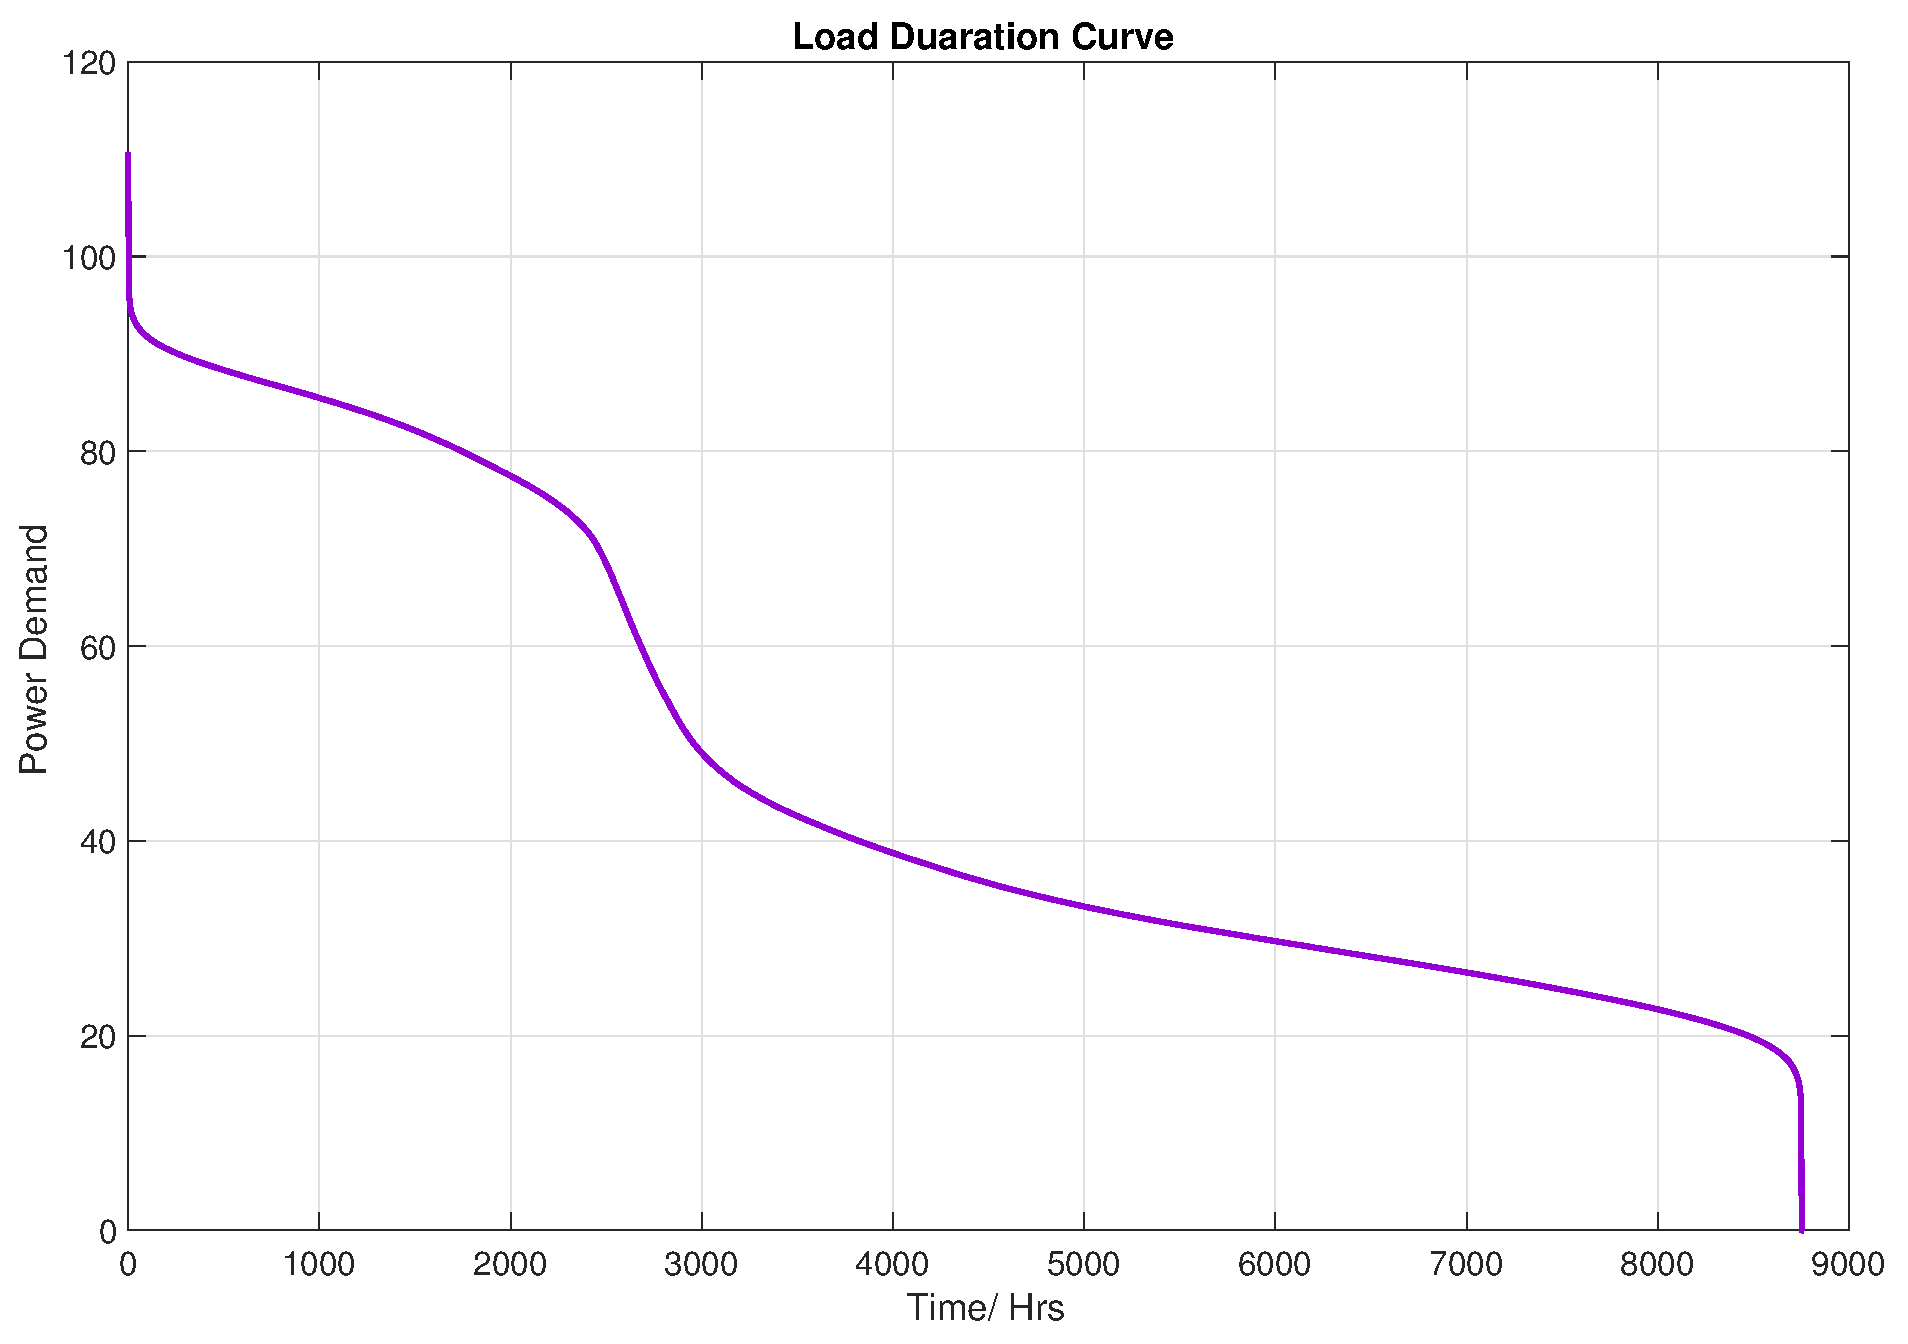
\includegraphics[trim = 0 0 0 0, clip, width=0.9\textwidth]{loadprofile.eps}
  \end{center}
  \caption{Load Duration Plot of Year Usage Data}
  \label{loadprofile}
\end{figure}

\subsection{Model Operation
Parameters}\label{model-operation-parameters}

The following Operational Parameters Were Used to Generate the Output
Results Discussed in this report. Values stated as variables were varied
per battery.

\begin{table}[H]
\begin{tabular}{p{4.3cm}p{8cm}}
\textbf{Upfront Costs}:& Variable\\
\textbf{Max Power}:& Variable\\
\textbf{Upfront Costs}:& Variable\\
\textbf{Depth Of Discharge \textit{(DoD)}}:& 80\% \\
\textbf{Cycle Life}:& 5000 [@TeslaPow57:online]\\
\textbf{Max Charge}:& $\frac{1-\text{DoD}}{2+\text{DoD}} \times$ CurrentCapacity\\
\textbf{Min Charge}:& $\frac{1-\text{DoD}}{2} \times$ Current Capacity\\
\textbf{End Life Value}:& 80\%\\
\textbf{Additional Costs}:& £0 \\
\textbf{Charge Rate}:& Max Power $\times$ 0.4 (In kWh per Half Hour)\\
\textbf{TRIAD Days}:& 04-Dec-2014, 19-Jan-2015, 02-Feb-2015\\
\textbf{TRIAD Rate}:& £33.55  (price per KW)\\
\textbf{Unit Rate}:&  6.832p\\
\textbf{Red Rate}:&  24.41p\\
\textbf{Amber Rate}:&  0.287p\\
\textbf{Green Rate}:&  0.161p\\
\textbf{Usage Variation $\sigma$}:&  $\frac{\text{Max Value + Mean Value}}{2}$ (For minute by minute granularity)
\end{tabular}
\label{inputparam}
\caption{Table Showing the Input Parameters of the Model}
\end{table}
% -----------------------------------------------------------------------------------
%                                  APENDIX
% -----------------------------------------------------------------------------------
\end{counted} %<<<<<<<<<<<<<<ENDS WORD COUNTER
Above were \thewords\ words. %<<<<<<<<<<<<<<DISPLAYS WORD COUNTER
% -----------------------------------------------------------------------------------
%                               BIBLIOGRAPHY - Insert Name of BIB File Here
% -----------------------------------------------------------------------------------
\newpage

% ---------------BIBTEX OLD-----------------------------------------------------
% \bibliographystyle{unsrt} %%%% Plain or alpha can change orders here
% \bibliography{BibFile}
% \nocite{*} %%%if you want to see all references even those note cited in the text
% -----------------------------------------------------------------------------------

\printbibliography

\end{document}
